\documentclass[12pt,a4paper]{article}

% \usepackage{array}
% \usepackage{pbox}
% \usepackage{hanging}
\usepackage{fancyhdr}
% \usepackage{caption}
% \usepackage{enumitem}
\usepackage{fancyvrb}
\usepackage{color}
\usepackage[utf8]{inputenc}
\usepackage{graphicx}
\usepackage{listings}
\usepackage{url}

\usepackage{xspace}

\usepackage{rotating}
\usepackage{wrapfig}

\usepackage{cite}
\usepackage{textcomp}

\usepackage[gen]{eurosym}
\usepackage{hyperref}

\usepackage{todonotes}

\usepackage{gensymb}

% \usepackage{draftwatermark}
% \SetWatermarkText{draft v2}
% \SetWatermarkScale{6}

\fancypagestyle{plain}{ %
  \fancyhf{} % remove everything
  \renewcommand{\headrulewidth}{0pt} % remove lines as well
  \renewcommand{\footrulewidth}{0pt}
}

\hyphenation{EISCAT}

\newenvironment{MYitemize}{%
    %% \renewcommand{\labelitemi}{$\rightarrow$}%
    %% \renewcommand{\labelitemii}{$\circ$}%
    %% \renewcommand{\labelitemii}{$\rightarrow$}%
    %% \renewcommand{\labelitemiii}{$\rightarrow$}%
    %% \renewcommand{\labelitemiii}{\colblack $\cdot$}%
    \begin{itemize}}{\end{itemize}}

\newcommand{\bitm}{\begin{MYitemize}}
\newcommand{\eitm}{\end{MYitemize}}

\newcommand{\N}{NeIC\xspace}
\newcommand{\NP}{NeIC~E3DDS\xspace} % NeIC project

\newcommand{\ED}{EISCAT\_3D\xspace}
\newcommand{\EC}{EISCAT\xspace}
\newcommand{\ESA}{EISCAT Scientific Association\xspace}
\newcommand{\SA}{sub-array\xspace}
\newcommand{\SAs}{sub-arrays\xspace}
\newcommand{\RS}{radar site\xspace}
\newcommand{\RSs}{radar sites\xspace}
\newcommand{\OS}{on-site\xspace}
\newcommand{\OC}{operations centre\xspace}
\newcommand{\CC}{control centre\xspace}
\newcommand{\DC}{data centre\xspace}
\newcommand{\DCa}{dCache\xspace}
\newcommand{\DCs}{data centres\xspace}
\newcommand{\UAF}{User Analysis Facility\xspace}

\newcommand{\RB}{ring buffer\xspace}
\newcommand{\fsru}{first stage receive unit\xspace}
\newcommand{\FW}{file writer\xspace}
\newcommand{\FIR}{Finite Impulse Response\xspace} 
\newcommand{\SBF}{second beam former\xspace}
\newcommand{\NNB}{$2 \times 100$\xspace} %number of narrow beams

\newcommand{\NBW}{5~MHz\xspace} % narrow bandwidth
\newcommand{\WBW}{30~MHz\xspace} % wide bandwidth

\newcommand{\ramf}{Ramfjordmoen\xspace}
\newcommand{\controllatency}{less than $5$\xspace}
\newcommand{\CP}{C/C++\xspace}
\newcommand{\DI}{DIRAC\xspace}
\newcommand{\DRF}{DigitalRF\xspace}
\newcommand{\HDF}{HDF5\xspace}
\newcommand{\IB}{Infiniband\xspace}
\newcommand{\IBtwo}{200\,Gb/s~\IB}
\newcommand{\Ru}{Rucio\xspace}
\newcommand{\einfra}{e-infrastructure\xspace}
\newcommand{\neinfra}{national e-infrastructure\xspace}
\newcommand{\WR}{White Rabbit\xspace}
\newcommand{\UAP}{User access portal\xspace}

\newcommand{\bfmust}{\xspace{\bf must}\xspace}
\newcommand{\bfshould}{\xspace{\bf should}\xspace}
\newcommand{\Bfmust}{\xspace{\bf Must}\xspace}
\newcommand{\Bfshould}{\xspace{\bf Should}\xspace}
\newcommand{\bfshall}{\xspace{\bf shall}\xspace}
\newcommand{\Bfshall}{\xspace{\bf Shall}\xspace}

\newcommand{\FirstBF}{\xspace{\bf Shall}\xspace}

\newcommand{\visroot}{isualiz}
\newcommand{\vis}{\visroot{ation}\xspace}
\newcommand{\vise}{\visroot{e}\xspace}
% \newcommand{\Vis}{{Visualization}\xspace}
\newcommand{\threed}{{3-dimensional}\xspace}
\newcommand{\GD}{{GUISDAP}\xspace}

\newcommand{\gps}{{Gbit/s}\xspace}

\newcommand{\np}{national provider\xspace}
\newcommand{\nps}{\np{s}\xspace}

\newcommand\EatDot[1]{}

\newcommand{\pc}{prompt computing\xspace}

%\newcommand{\NBW}{5~MHz} % narrow bandwidth
%\newcommand{\WBW}{30~MHz} % wide bandwidth


% \setlength{\topskip}{0mm}
\setlength{\headheight}{15pt}
% \setlength{\topmargin}{-5.4mm}
% \setlength{\textheight}{230mm}
\setlength{\textwidth}{180mm}
\setlength{\oddsidemargin}{-5.0mm}
% \setlength{\evensidemargin}{10.0mm}
% \setlength{\captionmargin}{7mm}

\title{
{\bf Deliverable Document 2} \\
On-site data processing simulation}
\author{E3DDS Team~\footnote{
Anders Tjulin (EISCAT) {\tt anders.tjulin@eiscat.se};
Ari Lukkarinen (CSC) {\tt ari.lukkarinen@csc.fi};
Assar Westman (EISCAT) {\tt Assar.Westman@eiscat.se};
Carl-Fredrik Enell (EISCAT) {\tt carl-fredrik.enell@eiscat.se};
Dan Johan Jonsson (UiT) {\tt dan.jonsson@uit.no};
Janos Nagy (NSC) {\tt fconagy@nsc.liu.se};
Harri Hellgren (EISCAT) {\tt harri.hellgren@eiscat.se};
Ingemar H\"{a}ggstr\"{o}m (EISCAT) {\tt ingemar.haggstrom@eiscat.se};
Mattias Wadenstein (UmU) {\tt maswan@hpc2n.umu.se};
% Roy Dragseth (UiT) {\tt roy.dragseth@uit.no};
John White (NeIC) {\tt john.white@cern.ch}}}

\date{\today}

\begin{document}

\pagestyle{fancy}
\lhead{\bf E3DDS project}
\rhead{\bf 2: Benchmarking software}

\maketitle
\par\noindent
\begin{minipage}{0.5\textwidth}
  
\includegraphics[scale=0.18]{NEIC_logo_screen_black.pdf}
  %\vspace{-0.09in}
\end{minipage}
\begin{minipage}{0.5\textwidth}
  \hfill
  %\includegraphics[scale=0.25]{EISCAT3Dlogo1.pdf}
  % New official logo with green text
  
\includegraphics[width=0.75\linewidth]{e3d-logo-green-500px}
\end{minipage}

\begin{center}
\begin{tabular}{|l|l|} \hline
\large \bf Date & \large \bf Comments \\ \hline
% \large 2018/06/19 & First draft started \\ \hline
\large July 4$^{\rm th}$ 2019 & Version sent to Anders \\ \hline
\large August 19$^{\rm th}$ 2019 & Version sent SG \\
\hline
\large October 17th 2019 & SG recommends update\\
\hline
\large Feb 19th 2010 & Second version to SG \\
\hline
\end{tabular}
\end{center}

\newpage
\tableofcontents
\newpage

\section{Executive Summary}
\label{exec-summ}

%\todo[inline]{Executive summary to be written at the end of the document writing process? Moved the current exec summary to introduction as that's what it was more like}

This document describes the deployment and testing of the \ED online data processing systems.
The \ED online data processing software stack is considered to be run on as generic computing hardware as possible. At the time of writing of this deliverable, hardware benchmarking and evaluation is in progress. 
What is clear is that fully virtual environments would create too much uncertainties to the performance of the online computing environment.  Therefore, the work here has been concentrated on bare metal solutions.
Evaluation work continues with the help of \ED software developers and deployment experts at the \nps.
Currently, a test system of multiple First Stage Receive Units and data simulator nodes that produce raw data, a fast Ethernet switch and an appropriately equipped test server is being installed at the Kiruna site.  This will allow a realistic test of the data production and export from an \ED site.

\section{Purpose}
\label{purpose}

The purpose of this document is to describe the simulated data processing chain of the upcoming \ED radar.
This document briefly describes each component in the data processing chain and the work required to deploy on the \neinfra{s}.

\subsection{Intended Audience}

The intended audience of this document is primarily the \ED project management and staff in order to understand what is complete and where more work is required in the data chain.
The operators of national \einfra{s} can also use this document to understand the requirements on hardware and networks in order to support \ED.

\section{Introduction}
\label{intro}
%Just a reminder, to be removed later
%\emph{Author(s): John}

The overall objective of the \ED Data Solutions (E3DDS) project is to simulate the data chain from the First Stage Receive Units (FSRUs), connected to the antennas, to the File Writers that write out the narrow beam data files to be sent to off-site storage. We also consider what we refer to as ``prompt computing'', which essentially is real-time processing of beamformed raw voltage data to obtain spectral data and real-time overviews.
The components of this whole data chain are to be created and deployed for benchmarking. 
Figure~\ref{fig-data-chain} shows the latest block diagram of the suggested \ED site computing, based on current experience and expected performance of the latest available hardware. 
Its parts are described in following sections. 
A test system will be installed at the Kiruna site. 
Resources at national \einfra provider partners of the project are also being explored for file transfer and user analysis tests.

This document describes the components and work for the on-site data processing software environment.
The most essential components discussed in this document are simulation software for the data output from the FSRUs: the prototype software for Second Beam Former (SBF), and a file writing software. 

The object to be delivered consists of a description of the prototype software(s) and any available benchmark results. 
% \todo[inline]{link to summaries of benchmarks, both those running in the \einfra of the \nps and on the AMD test server}.  

\begin{figure}[h!]
\centering
%% 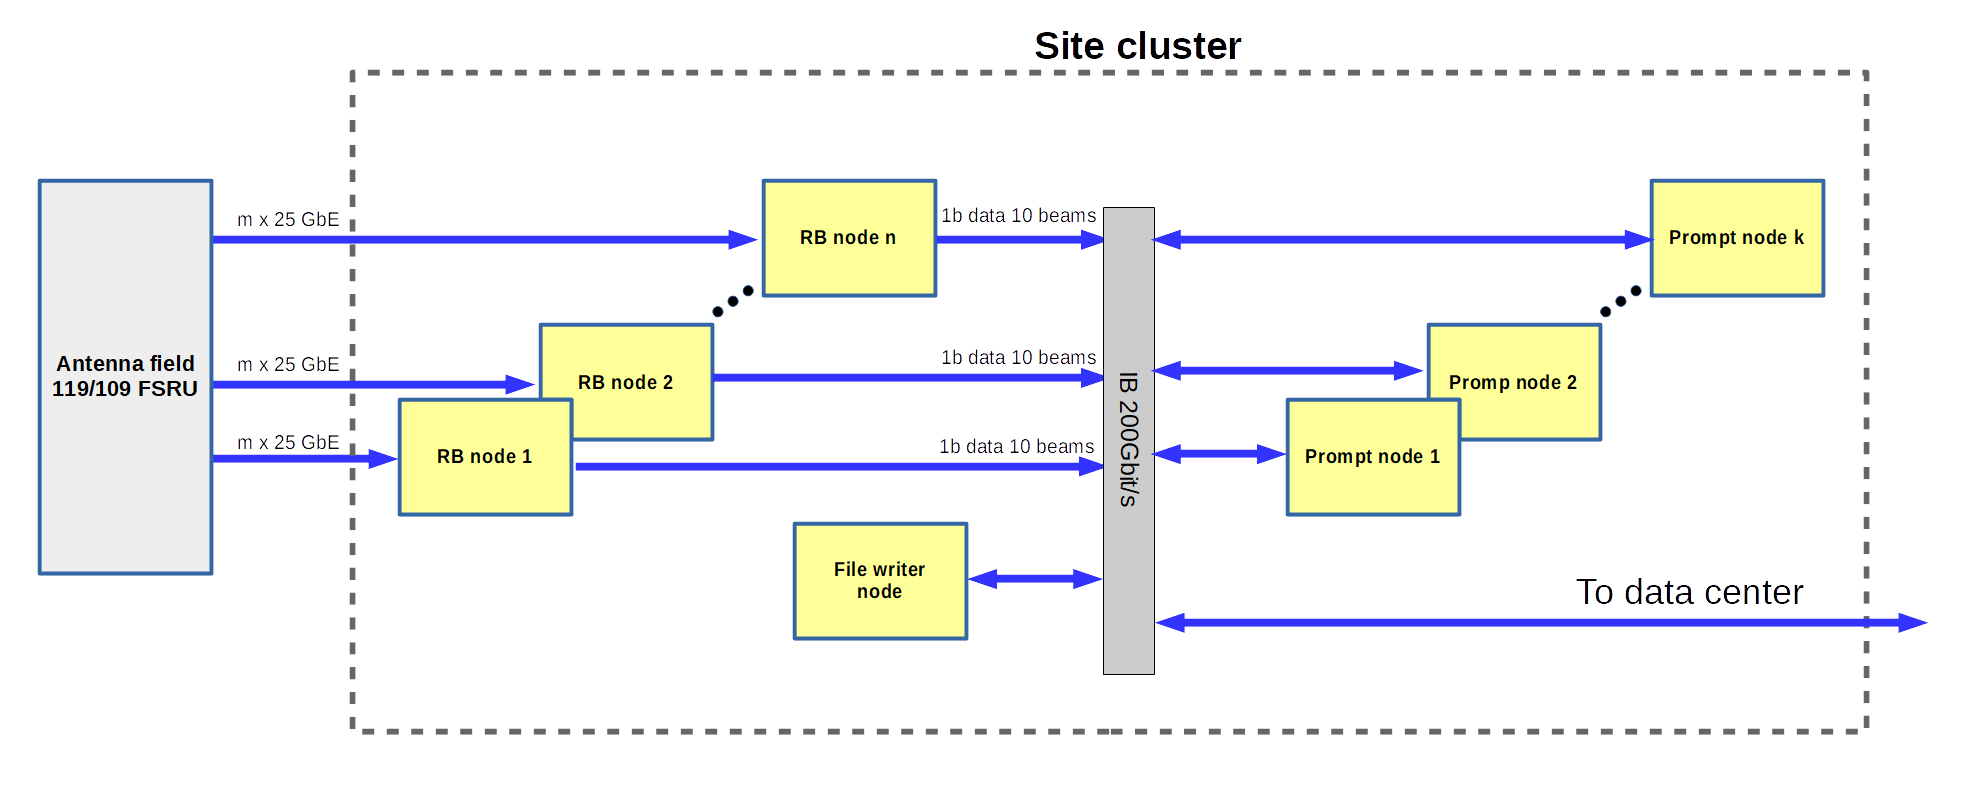
\includegraphics[scale=0.3]{E3DDS_D2_data_flow.png}
%% 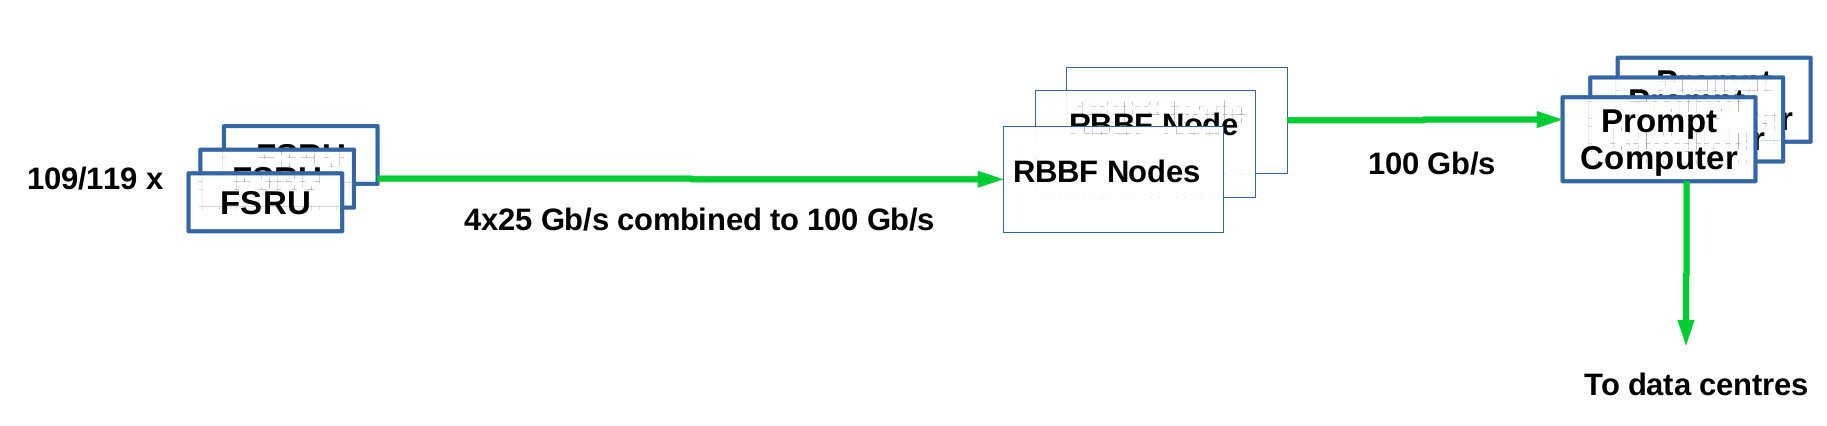
\includegraphics[scale=0.35]{E3DDS_D2_figure1.png}
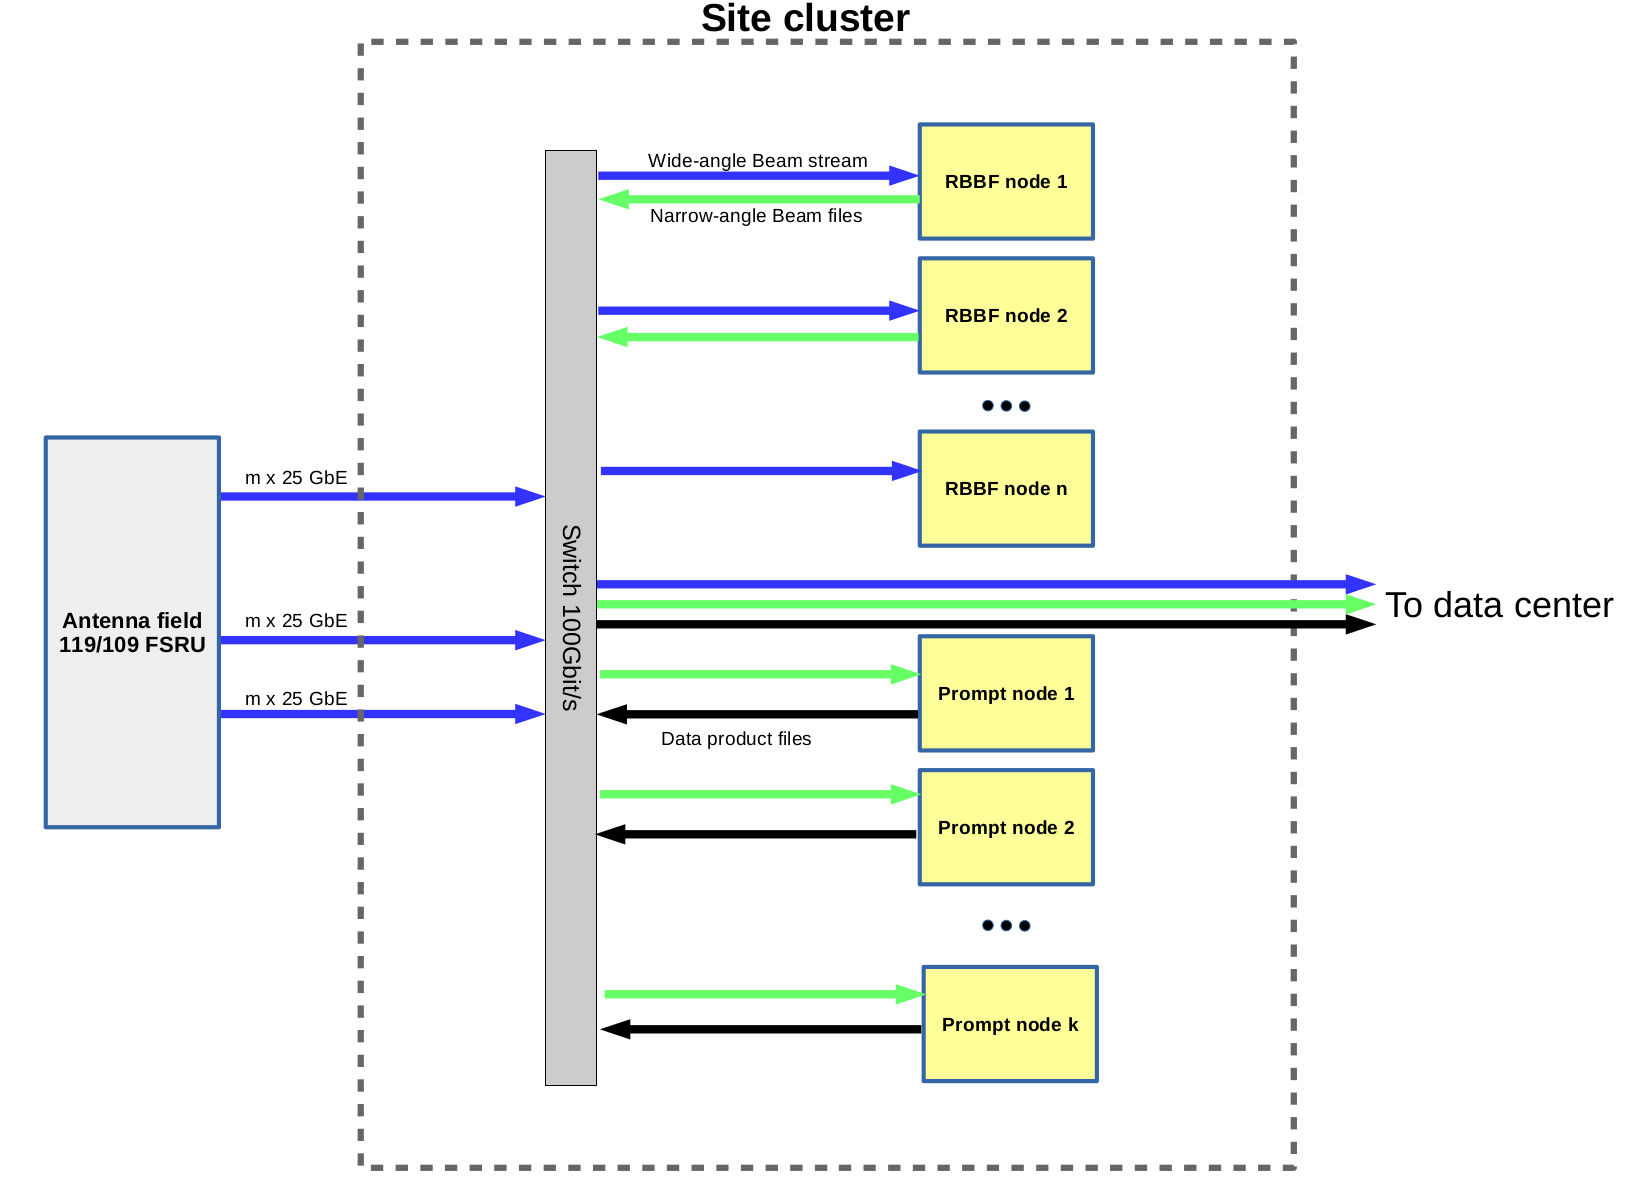
\includegraphics[scale=0.35]{E3d_data_flow_modified.png}
\caption{
% \todo[inline]{Carl-Fredrik: New diagram from Harri: ethernet switch and combined RBBF nodes}
The data flow from FSRUs; data is streamed from the FSRUs to Ring Buffer Beam Former (RBBF) nodes and onwards to the prompt computing that produces the basic scientific data products. Alternatively, any data level may be written to storage buffers at a data centre.\label{fig-data-chain}}
\end{figure}

\section{Multi-site radar control}
%\todo[inline]{Should this section be moved up? Done}
The control system taking care of all \ED sites is a crucial and complicated part of the software to be built. 
The main principle of the design is to use a relational database for configurations as well as for other statistical data and a messaging system for system commands and dynamically changing data. 

\subsection{System description}

The multi-site control system consists of independent processes which are running in the Operations Centre and on site management cluster computers, see Section~ \ref{sec:onsitemanagementcluster}. Communication between modules is performed using a messaging system. 

\begin{figure}[h!]
\centering
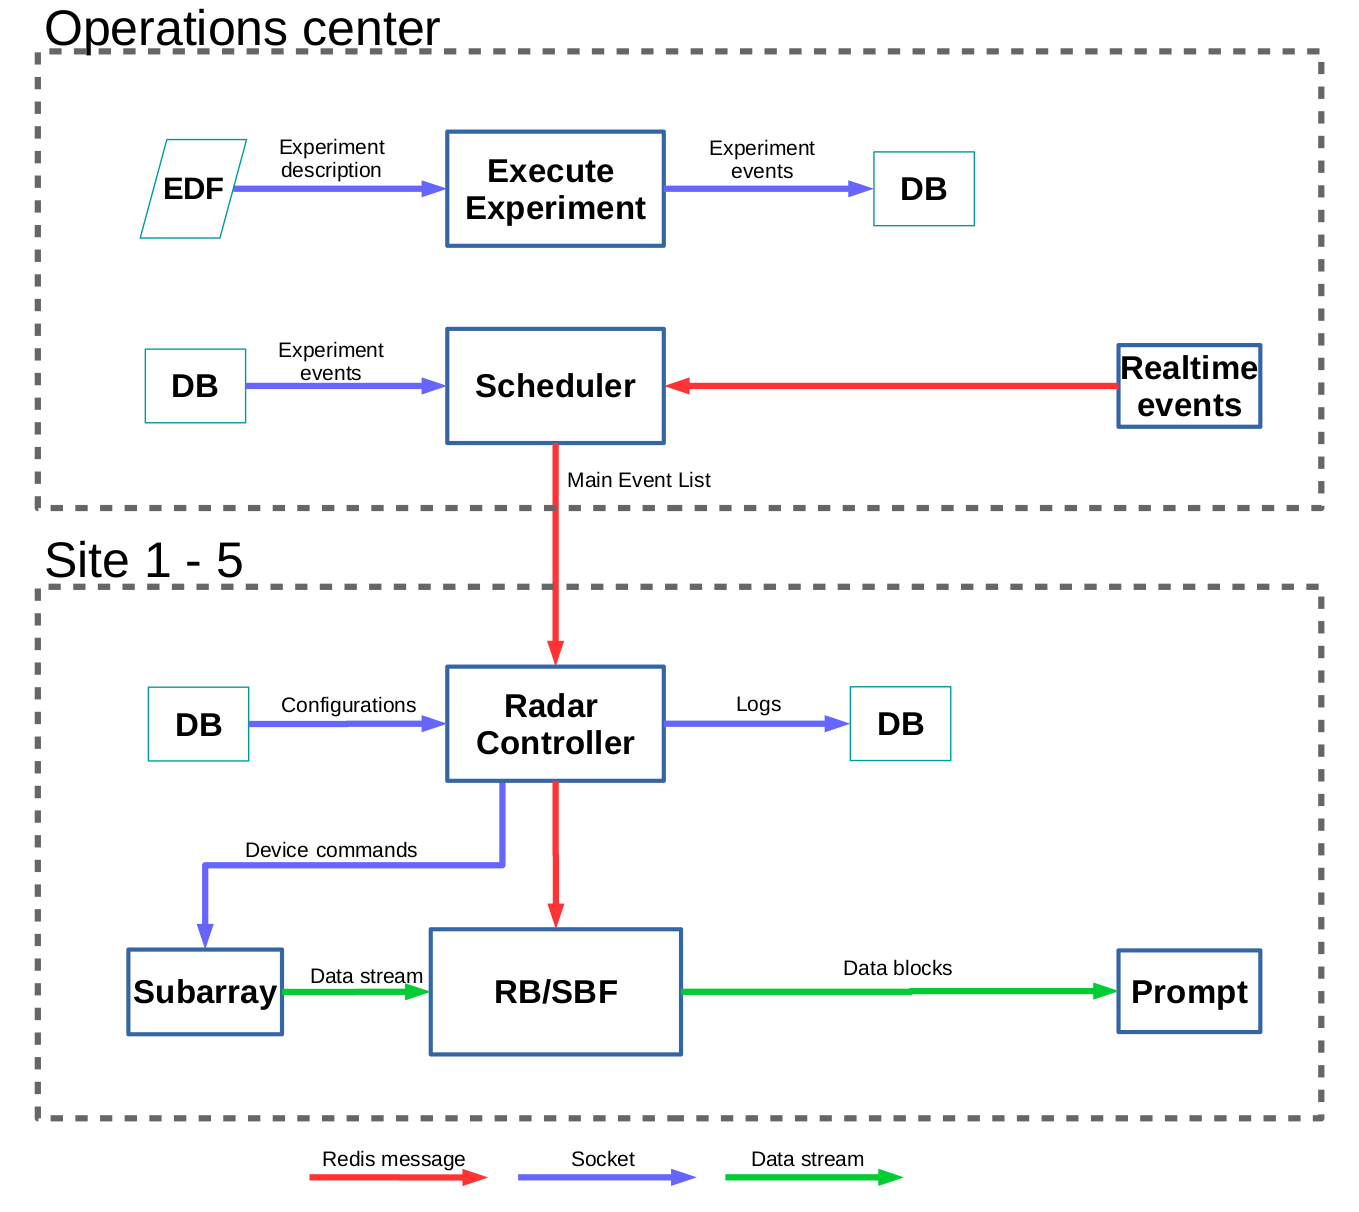
\includegraphics[scale=0.4]{do2_figure2.png}
\caption{Multi-site Control System \label{fig-control-sys}}
\end{figure}

Users create experiments description file (EDF) using web interface or Matlab/Python scripts and upload to the \ED  database through a secured web interface. 
The operator accepts which experiment are executed and a process for each is started. 
The experiment description is then translated to detailed events. 
An event is a set of commands that will control the \ED hardware. 

A \emph{Scheduler} process selects which events are executed at a given time and builds up a {\emph{Main Event List}} which is continuously generated and streamed to the radar controllers at each site.  

\subsection{Relational database}

Some relational databases are available and the choice between may be difficult. 
The E3DDS project, however, recommends to use the PostgreSQL database~\cite{postgresql}, which is one of the most widely used databases. 
At the moment there are not any special requirements for the database which should drive the database selection towards any more specialized product.

\subsection{Messaging system}
The aim of the fast control system is to be able to change radar operation parameters within a few seconds timescale. 
During this time, data has to be received, analyzed, decision made to change the radar parameters, new parameters calculated, and new commands send to all sites. 

A number of suitable messaging systems are available and after some testing E3DDS recommends Redis~\cite{redis}. Redis is an open source (BSD licensed), in-memory data structure store, used as a database, cache and message broker. 
Redis has been tested as a message broker and in-memory cache. 
% Do we have results available? JSW
% Check with Assar.


\section{FSRU Data stream}


\subsection{FSRU data structure}

The data stream output from the FSRU has been defined in collaboration with the supplier~\cite{da-design}. 
The UDP protocol was chosen for a minimal header size and complexity.  
The packet structure is:
\begin{center}
\begin{tabular}{cl}
\multicolumn{2}{l}{\textbf{Bytes Description}} \\
                0--19 	& IPv4-header (no options) \\
                20--21 	& UDP-header –- Source port (fixed) \\
                22--23 	& UDP-header –- Destination port (configured via control protocol) \\
                24--25 	& UDP-header –- length: 9562 (0x255A) \\
                26--27 	& UDP-header –- checksum (0x0000 –- not used) \\
                28--29 	& Pad (0x0000) \\
                30--33 	& Beam index \\
                34--37 	& Data packet index \\
                38--45 	& Time stamp of the beams first sample (Data packet index 0 sample 0) \\
                        & 64-bit unsigned integer seconds from epoch \\ % Question about 64-bit timestamps. JSW
                46--48  & 	Microseconds part of the timestamp (24-bits) \\
                49 	 & Sample clock cycles from the previous 1 $\mu$s  mark (0 – 103) \\
                50--53 &	Packet flags  \\
                54--55 &	Beam Q-data 0 \\
                56--57 &	Beam I-data 0 \\
                58--59 &	Beam Q-data 1 \\
                60--61 &	Beam I-data 1 \\
                ... -- ... &	Beam Q-data 2381 \\
                9580--9581 &	Beam I-data 2381 \\
\end{tabular}
\end{center} 

\subsection{Network}
The current understanding is that data streams from all subarrays will be sent to the compute nodes via high-speed (100 Gb/s full duplex) Ethernet switches. In this way the data packets from the same beam direction of every subarray can be routed to a single compute node, facilitating the computations. 
                
\subsection{FSRU Emulator}
A UDP packet data emulator was implemented using MoonGen~\cite{moon-gen} software. 
MoonGen is a fully scriptable high-speed packet generator. It features multi-core support, precise time-stamping and rate control. 

A test script to simulate a full rate of one FSRU packet stream was done and tested. This will be feed through a 100 GbE switch and to an AMD EPYC server~\cite{amd-epyc}. 

For further benchmarking of the \SBF{} node, we will use two high performance gaming PCs with AMD Ryzen CPUS running the MoonGen emulator to feed data packets to the system. Additionally the \fsru{} first article will be used when available.

\section{Compute nodes}
%\section{Ring buffer functions}
%Just a reminder, to be removed later
%\emph{Author(s): Harri, Simon}
%- available C/C++ libraries
%- interface, API
%- intrupts from NIC
%- call backs to SBF
%- benchmarking


During the course of the project some different options for the ring buffer architecture have been considered, including
% Nodes are connected between receiver (FSRU) and second beam former nodes.
connecting the \fsru{} 25~GbE outputs directly to the \RB nodes without using an Ethernet switch. 
All \RB{} nodes and \SBF{} nodes would then have to be connected together using an Infiniband switch.  This assumed that the \SBF{} would be based on true time delays implemented as \FIR{} filters. Later it was seen that beamforming at \NBW{} can be handled by applying time delays only in the \fsru{}s followed by simple phase multiplications in the \SBF{} (Figure~\ref{phase-steering}). This allows \RB and \SBF processes to run on the same nodes and simplifies the architecture considerably. Our suggested architecture is thus to deploy combined ring buffer and \SBF{} server nodes.  Data from the \fsru{}s will flow through 100 Gb/s Ethernet connections.

The \RB + \SBF node, as shown in Figure~\ref{fig-rb-node}, then consists of following parts:
\begin{itemize}
\item Two or more 100 Gbit/s network cards (NIC);
\item Ring Buffer Writer (RBW);
\item Second Beam Former  (SBF);
\item Ring Buffer (RB);
\item Event Writer(EW);
\item Fast access storage (SSD).
\end{itemize}

\begin{figure}
\centering
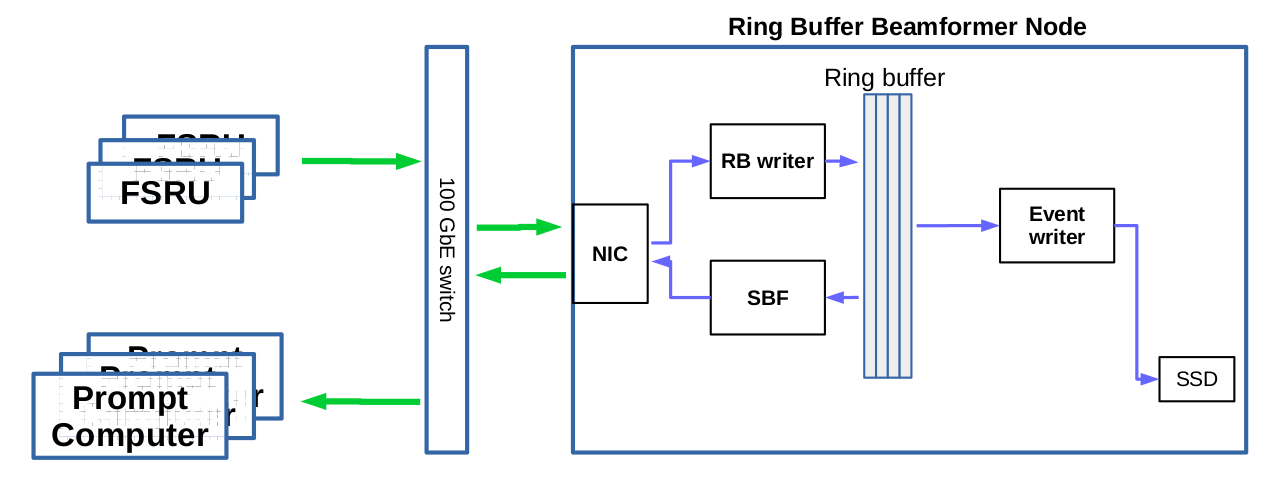
\includegraphics[scale=0.4]{E3DDS_D2_RBBF_Node.png}
\caption{% \todo[inline]{Harri's new diagram with switch and SBF running on RB node here}
Schematic of the proposed Ring Buffer Beam Former (RBBF) Node. \label{fig-rb-node}}
\end{figure}

\section{Ring buffer functions}

\subsection{Operation modes}
During the project, the following operation modes have been recognized:
\begin{itemize}
\item Normal (nominal) operation;
\item Fast saving;
\item Saving all to SSDs;
\item Partial saving to SSDs.
\end{itemize}

\subsubsection{Nominal operation}

In the nominal operation mode, shown in Figure~\ref{rb-normal-operations}, UDP packets are received and transferred to the ring buffer RAM. 
In the ring buffer, UDP packets form a larger data structure which is then forwarded to the \SBF process. 
It is expected that the \NBW bandwidth, that corresponds to a nominal sample rate of 6.5 Mega Samples Per Second (MSPS), can be executed in real time. 

\begin{figure}[h]
\centering
%% 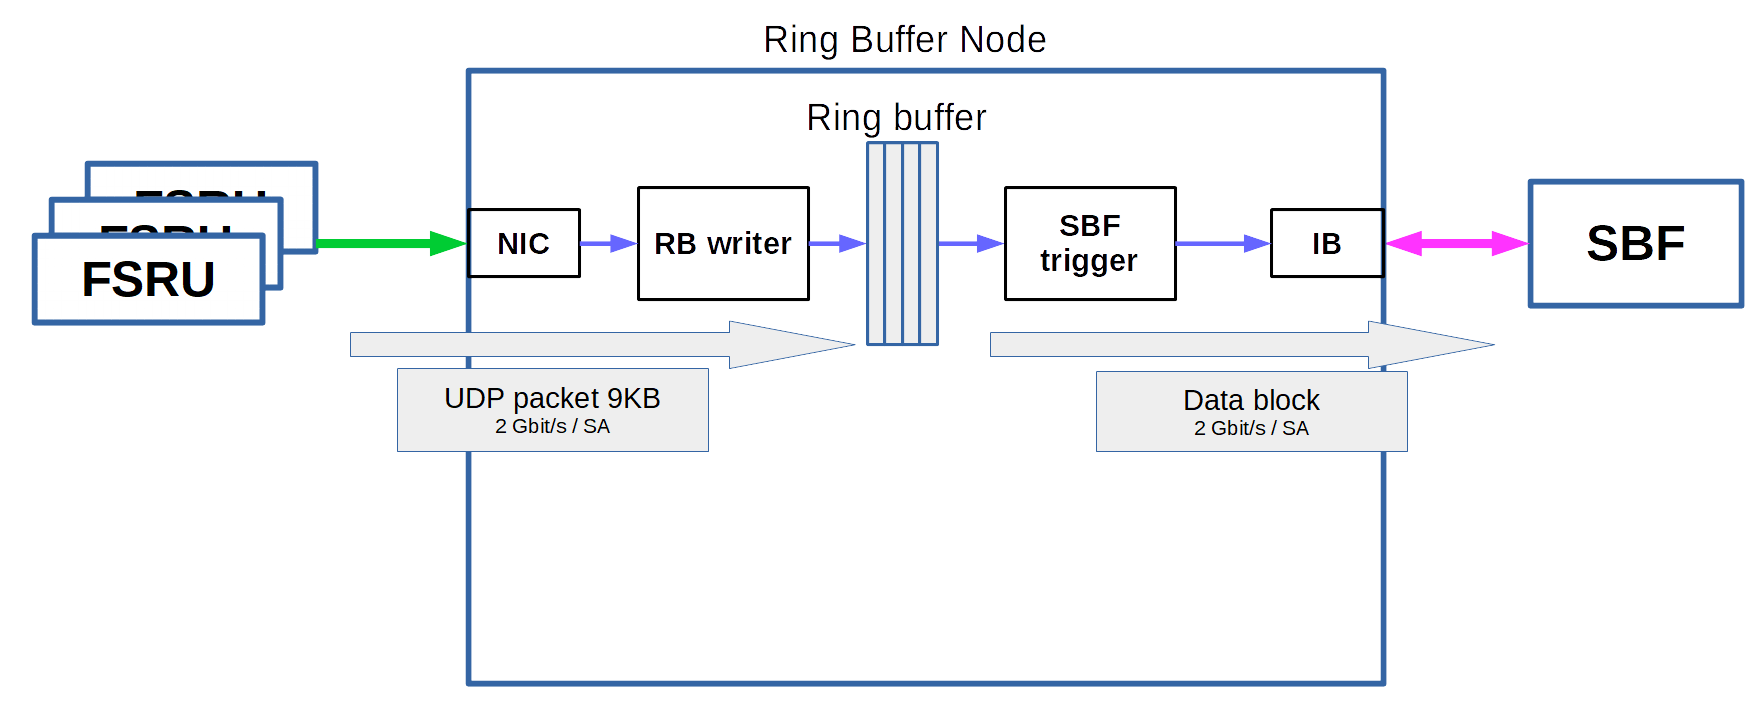
\includegraphics[scale=0.5]{E3DDS_D2_RBN_normal_op.png}
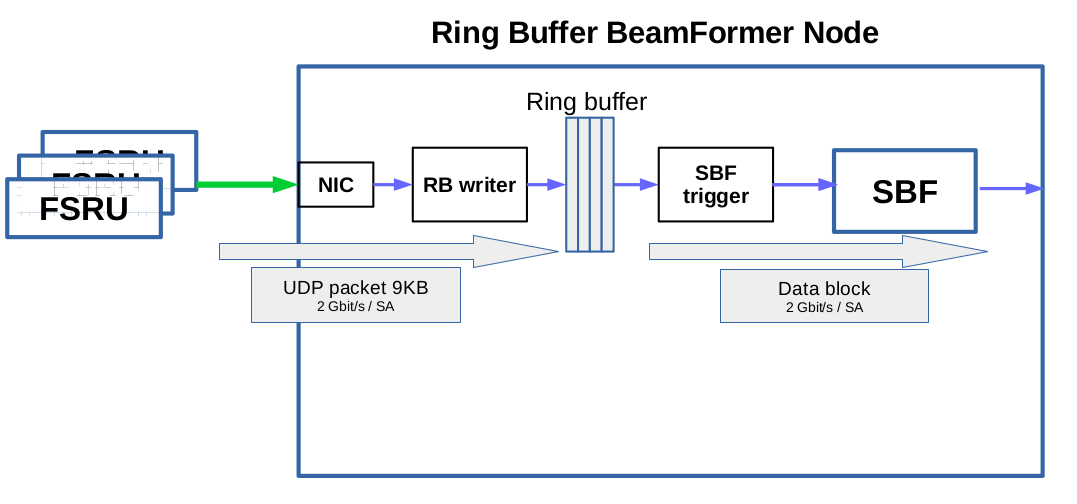
\includegraphics[scale=0.4]{E3DDS_D2_RBBF_Node_fig4.png}
\caption{
% \todo[inline]{Harri's new diagram with switch and SBF running on RB node here}
Raw (level 1) data is buffered to RAM and subsequently read by the SBF.\label{rb-normal-operations}
}
\end{figure}

\subsubsection{Fast saving}
When operating in the \WBW mode, the full sample rate from each FSRU is 52 MSPS, which the RB nodes must be able to save to the memory. 
In this mode UDP packets are only saved the ring buffer in real time and all other operations are done later, as shown in Figure~\ref{rb-fast-save}. 
In this way the full performance of the FSRUs can be used but the narrow beams (from the second level beam former) are not required to be calculated at this data rate. 
\begin{figure}[h]
\centering
%% 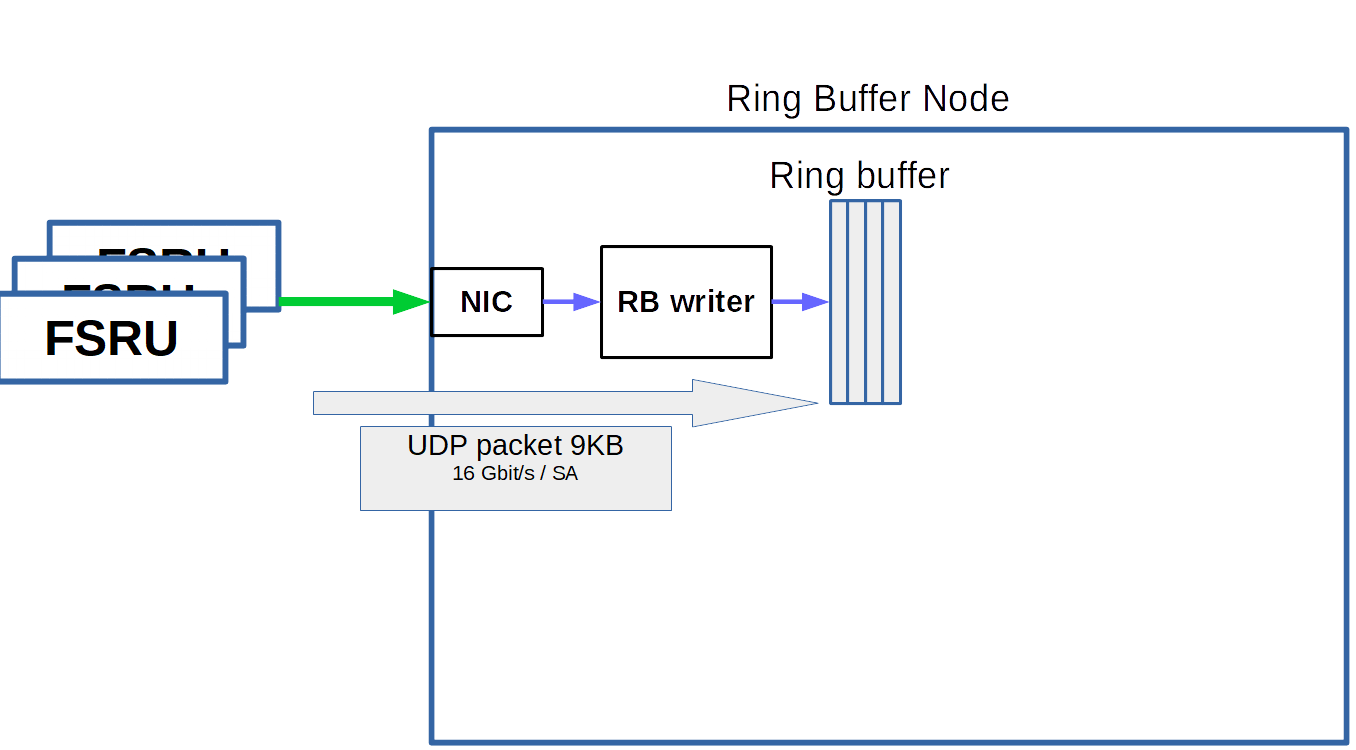
\includegraphics[scale=0.5]{E3DDS_D2_RBN_fast_op_cropped.png}
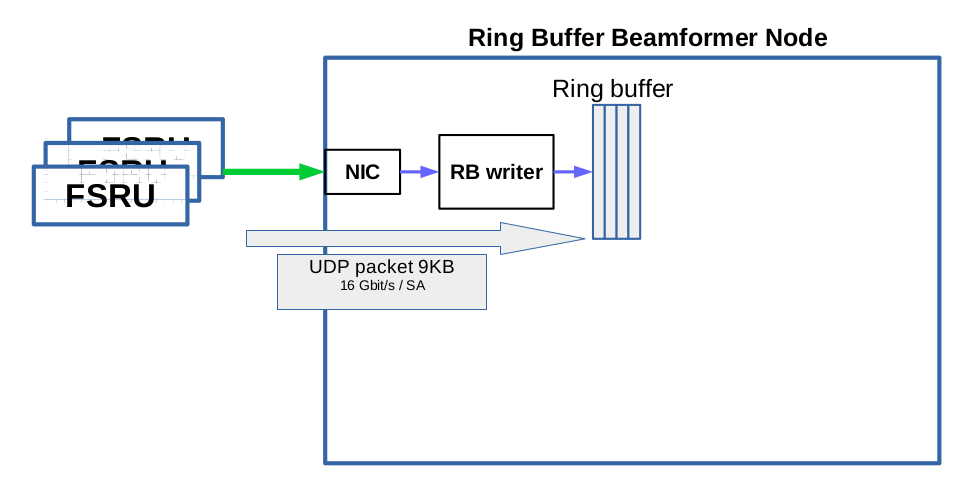
\includegraphics[scale=0.5]{E3DDS_D2_Figure_5.png}
\caption{
% \todo[inline]{Harri's new diagram with switch and SBF running on RB node here. Or show only the node not the network.}
Raw (level 1) data is saved directly to RAM in the RBBF node.\label{rb-fast-save}
}
\end{figure}

\subsubsection{Raw data saving}
For longer but wide band (6.5~MSPS) experiments we have decided to add fast SSD disks for raw data storage. UDP packets are written to ring buffer but instead of transferring them to the second beamformer, data is saved to fast NVMe SSDs attached to the node as shown in Figure~\ref{rb-raw-data-save}.
\begin{figure}[h!]
\centering
%% 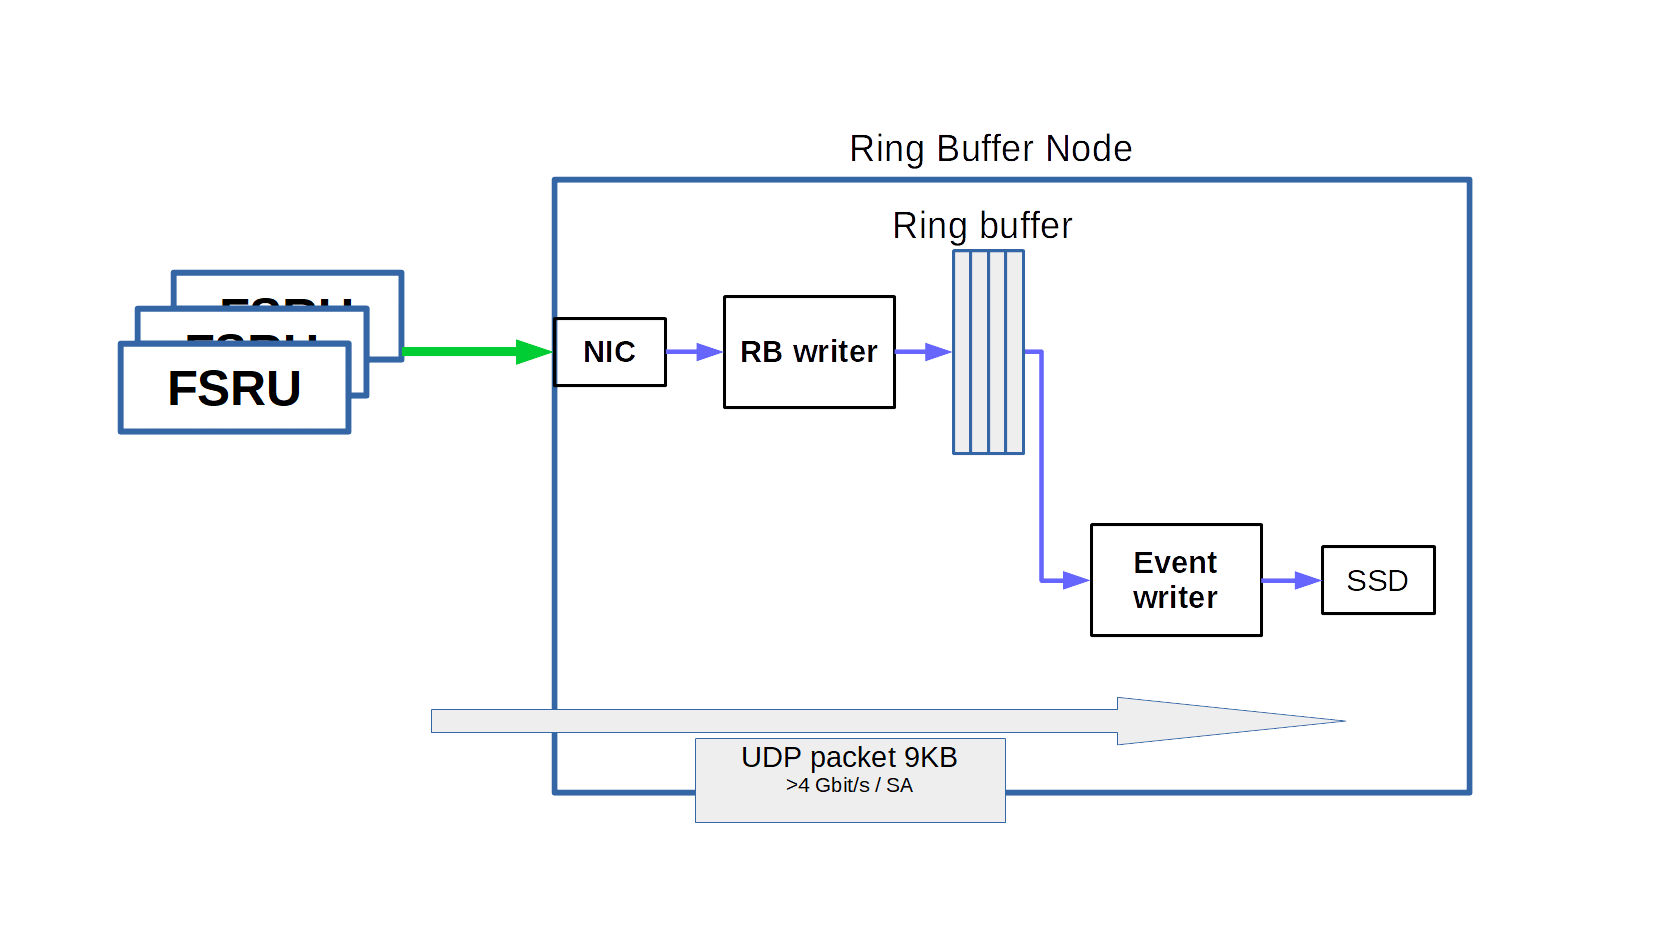
\includegraphics[scale=0.5]{E3DDS_D2_RBN_raw_save.png}
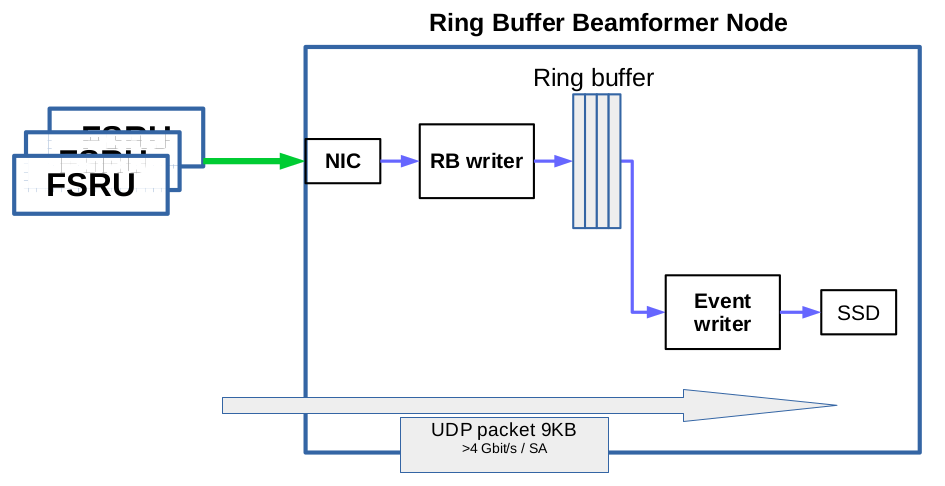
\includegraphics[scale=0.5]{E3DDS_D2_Figure_6.png}
\caption{
% \todo[inline]{Harri's new diagram with switch and SBF running on RB node here. Or show only the node not the network.}
Raw (level 1a) data is saved directly to the SSD(s) in the RBBF node.\label{rb-raw-data-save}}
\end{figure}

\subsubsection{Raw data partial saving}
During normal operation, part of the \fsru{} data can be saved to SSDs. This operation may slow down processing and in any case cannot be done continuously due to SSD lifetime.
It has been estimated that about 1~\% of level~1 data (see Table 1 in~\cite{e3dds-del1}) shall be saved for long-term archival in this operation mode.
% \todo[inline]{Carl-Fredrik: when we say raw data archival do we really mean to save 1\% of level 1a data, or are we talking only about  beamformed 1b data to archive?}

\section{Second level beamforming}
\label{sec:sbf-phase}

% \section{Second beam former}
%Just a reminder, to be removed later
%\emph{Author(s): Assar, Dan, John}

The \ED second level beam former (SBF) produces the final narrow angle beams as detailed in~\cite{assars-note}.
%One of the components needed in the second level beam former is a fast Finite Impulse Response (FIR) filter %which adds the necessary time delay on every beam that comes from the first level beam former 
%out in the antenna array. 
% The number of beams output from the first level beam formers are $109 \times 10 \times 2 = 2180$. 
There will be 2180 beams coming out from the first level beam former (109 sub-arrays, with 10 beams each in 2 polarisations).
%On all of these data streams an individual FIR 
%filter must be applied and the results added together to form a beam using all the array antennas. During the %operation, SBF should also change integer values to floating points. 
The required process has been evaluated using several candidate technologies.
\subsection{CPU}

Full FIR filtering using CPUs would require many nodes, as evident from the benchmarks as found in~\cite{assars-note}. The chosen approach of \fsru{} delays and phase multiplications is much faster and feasible to run on CPUs.  Currently we are about to start benchmarking a newly acquired AMD EPYC server~\cite{amd-epyc}. 
Forming 10 narrow beams out of the corresponding wide beams from every subarray is expected to be possible on a single dual CPU node, thus reducing the cluster size for the the \RB{} and \SBF{} functionalities to 10~nodes.

%The FIR filter may be applied using CPUs in servers.
%The FIR-filtered results must be summed to form the narrow beams.
%This may be performed within a server by sending all results for each narrow beam to be summed.
%Alternatively, this can be performed in a high-performance network \emph{e.g.} Infiniband when equipped with %the correct libraries~\footnote{See Mellanox SHARP\texttrademark technology,  \url{http://www.mellanox.com/page/hpcx_overview}.}.

%\todo[inline]{Need input from Dan on summations...}

\subsection{GPU}

Servers equipped with GPU(s) is an attractive choice as those can be programmed relatively easy and can be used for other purposes than only for beam forming. 
However, our tests have shown that the needed number of nodes to host the GPUs is still comparable to that for the CPU solution. 
The bottleneck is the data transfer rates to and from the memory of the GPUs.  
There is less of a data transfer bottleneck in IBM Power systems, as NVLink~\cite{nvlink} is used as a direct connection between GPUs.
This technology is not yet available from other vendors.

Currently we are evaluating GPUs attached to PCIe v4 for prompt computing tasks. They may be an attractive option for lag profiling and realtime analysis. It is therefore likely that a number of nodes with GPUs will be added to the site clusters.


\subsection{FPGA}

FIR filter calculations may be performed using dedicated hardware as is done in First Level Beam Former using Field-Programmable Gate Array (FPGA) hardware.  This would be the most efficient way but on the other hand it will be difficult to use the expensive hardware for other purposes, such as user analysis. 
Dedicated FPGA hardware deployed in servers could still be a future option for beamforming and sub-beam imaging at high bandwidths but will not be further considered here.

\subsection{FSRU}
\label{ssec-fsru}

The solution we have decided upon makes use of the FPGAs on the FSRUs to perform the long delays needed between sub-arrays, essentially shifting the start time of each beam. The summation of the results and a small phase change \emph{i.e.} complex multiplication can then be performed in the combined \RB and \SBF nodes.
Simulations made by Jussi Markkanen, shown in Figure~\ref{phase-steering}, show that the maximum error is about 0.2\degree\xspace  in beam pointing direction compared to time delay steering. This error can be seen only at $\pm$ 15~MHz out of reception center frequency. The beam width is simulated to be in order of 0.6\degree\xspace so the error can be considered to be small enough for this approach to be used. 
\begin{figure}[h!]
\centering
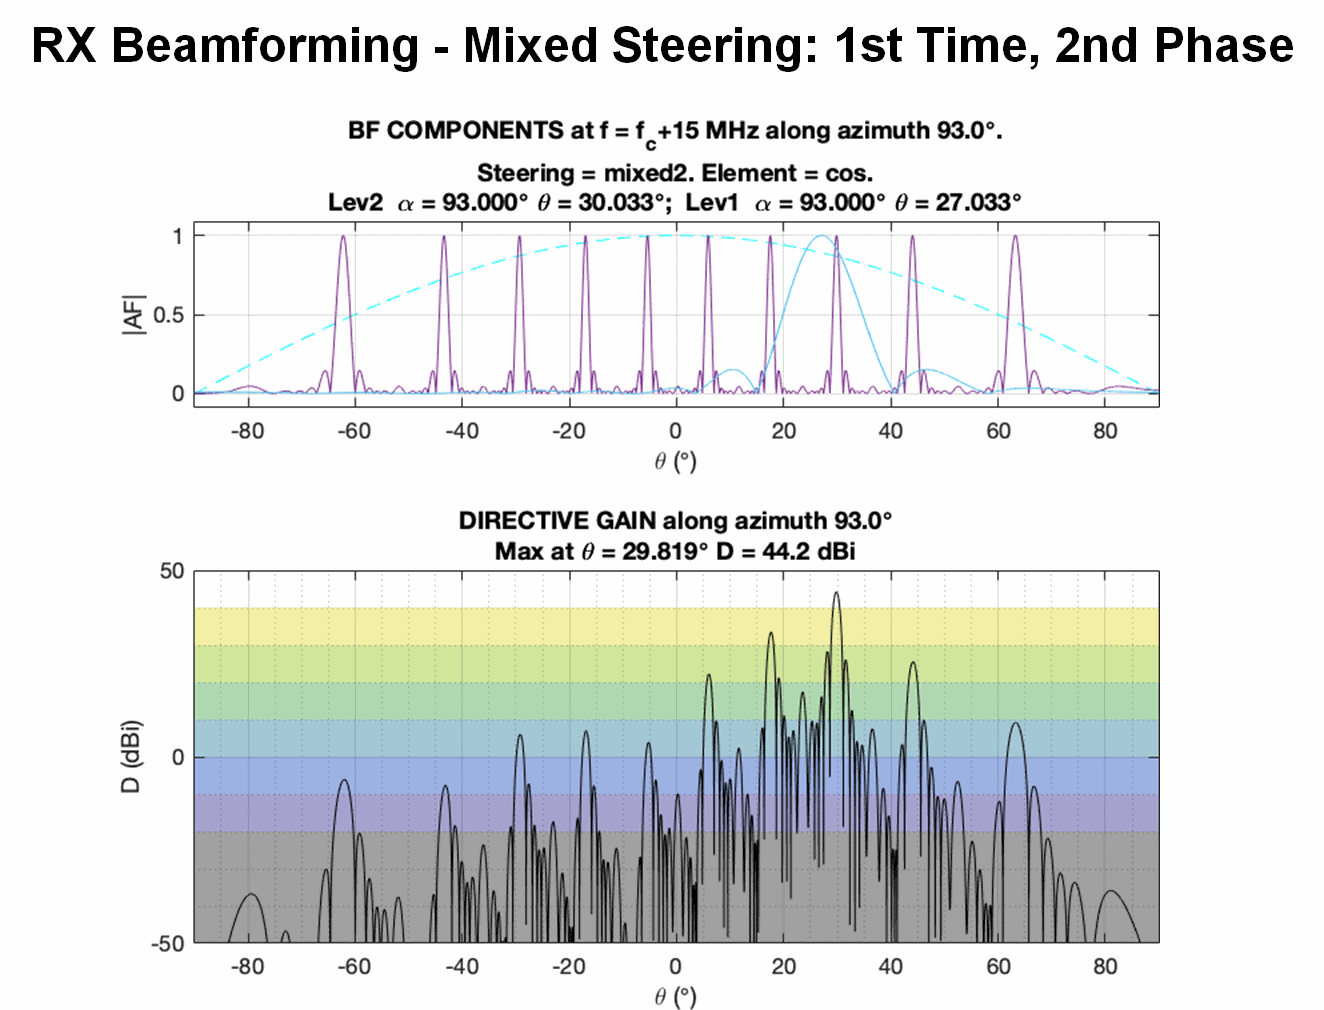
\includegraphics[scale=0.5]{E3DDS_D2_phasesteering.png}
\caption{Beam steering with separate time and phase calculations. \label{phase-steering}}
\end{figure}

\iffalse
\section{Propositions for hardware configuration}

The data throughput values in different operating modes have to be considered when deciding the Ring Buffer hardware configuration.
% Ring Buffer node hardware configurations has to be done looking data throughput values in different operating modes. 
The first consideration is how many 25 GbE optical lines can be connected to one ring buffer node. 
In the Fast Saving mode all FSRUs are sending data packets in full 52 MSPS speed. 
This data stream should go to the ring buffer in main memory. 

The latest AMD EPYC 7000 processors have memory bandwidth in order of 170 GB/s (1360 Gbit/s).
If all that can be used for data throughput, it means that the nominal data from FSRUs can be saved. 
So memory bandwidth should not be a bottleneck~\footnote{The next version of the AMD CPU is expected to provide PCIe Gen4 as well as even better memory bandwidth, see {\url{https://www.servethehome.com/why-amd-epyc-rome-2p-will-have-128-160-pcie-gen4-lanes-and-a-bonus/}}}.  
One PCIe Gen3 x16 connection can handle approximately 100~Gbit/s traffic. 
In the case of AMD EPYC 7000 series there 128 lines available. 
This means in theory 800~Gb/s traffic and about 48 FSRU full speed connections.

In practice we can consider to connect 12 FSRUs to each Ring Buffer node using three PCIe cards having four times 25 GbE connections each. 
This will be 66~Gb/s data stream in one PCIe x16 and about half of available bandwidth. 
The traffic to the main memory is then 200~Gb/s, which is only 1/6 of full available bandwidth.  

For the Fast Saving mode we need preferably latest Non-Volatile Memory Express (NVMe) M.2 SSD disks installed directly to the server board. 
For example the Samsung EVO Pro SSD has a sequential write speed over 3~GB/s (24~Gb/s) and thus can handle the nominal 6.5 MSPS (2~Gb/s) traffic from 12 FSRUs. 
%% Is this number above correct? Surely 6.5 MSPS x (16+16) bits x 2 pol = 416 Mb/s per FSRU. 12 FSRUs give 5 Gb/s ?
%% It's only one polarization. At this stage HW is divided to two parts and polarizations are combined only before lag-profile calculations.
The HighPoint SSD7120 SSD device is a PCIe x16 card which can be equipped with four M.2 SSDs in RAID 0 mode. This gives write speed of 12~Gbit/s (100~Gb/s) and in theory can handle traffic from 12~FSRUs having 17~MSPS decimated output rate.
\begin{figure}[h!]
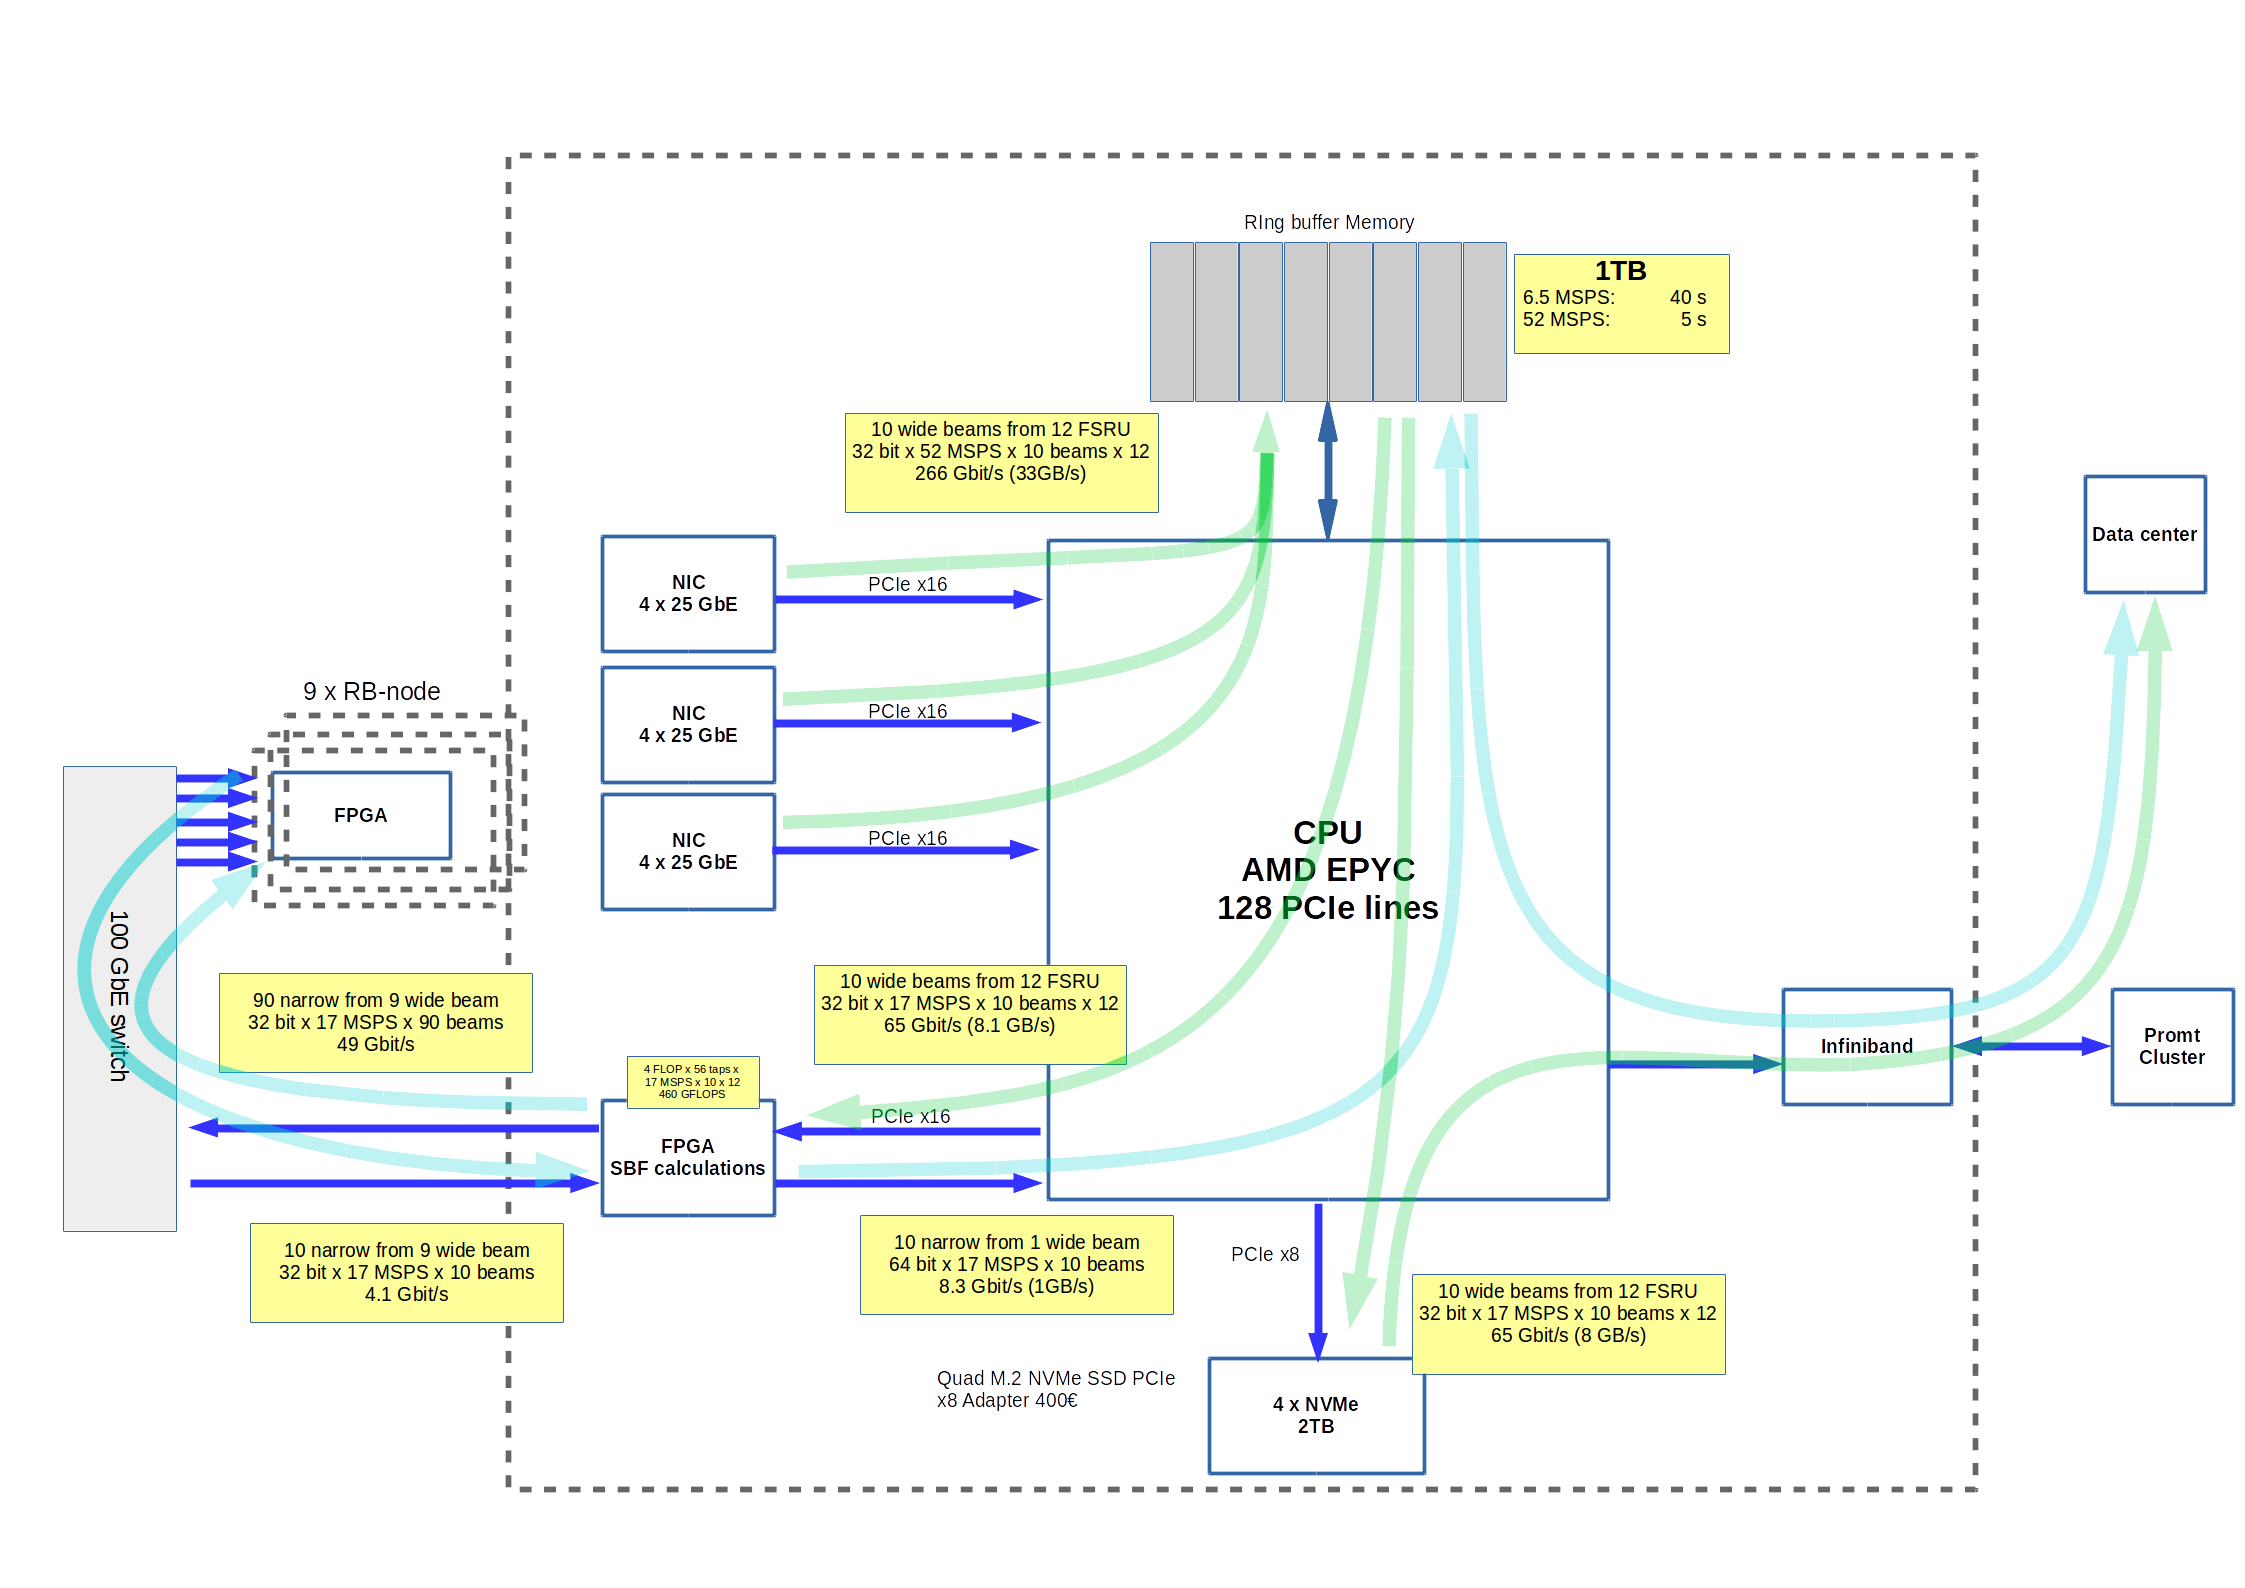
\includegraphics[scale=0.3]{E3DDS_D2_ring_buffer_node_dataflows.png}
\caption{An example of a possible hardware configuration with FPGA accelerators for Second Beam forming.}
\end{figure}
%% 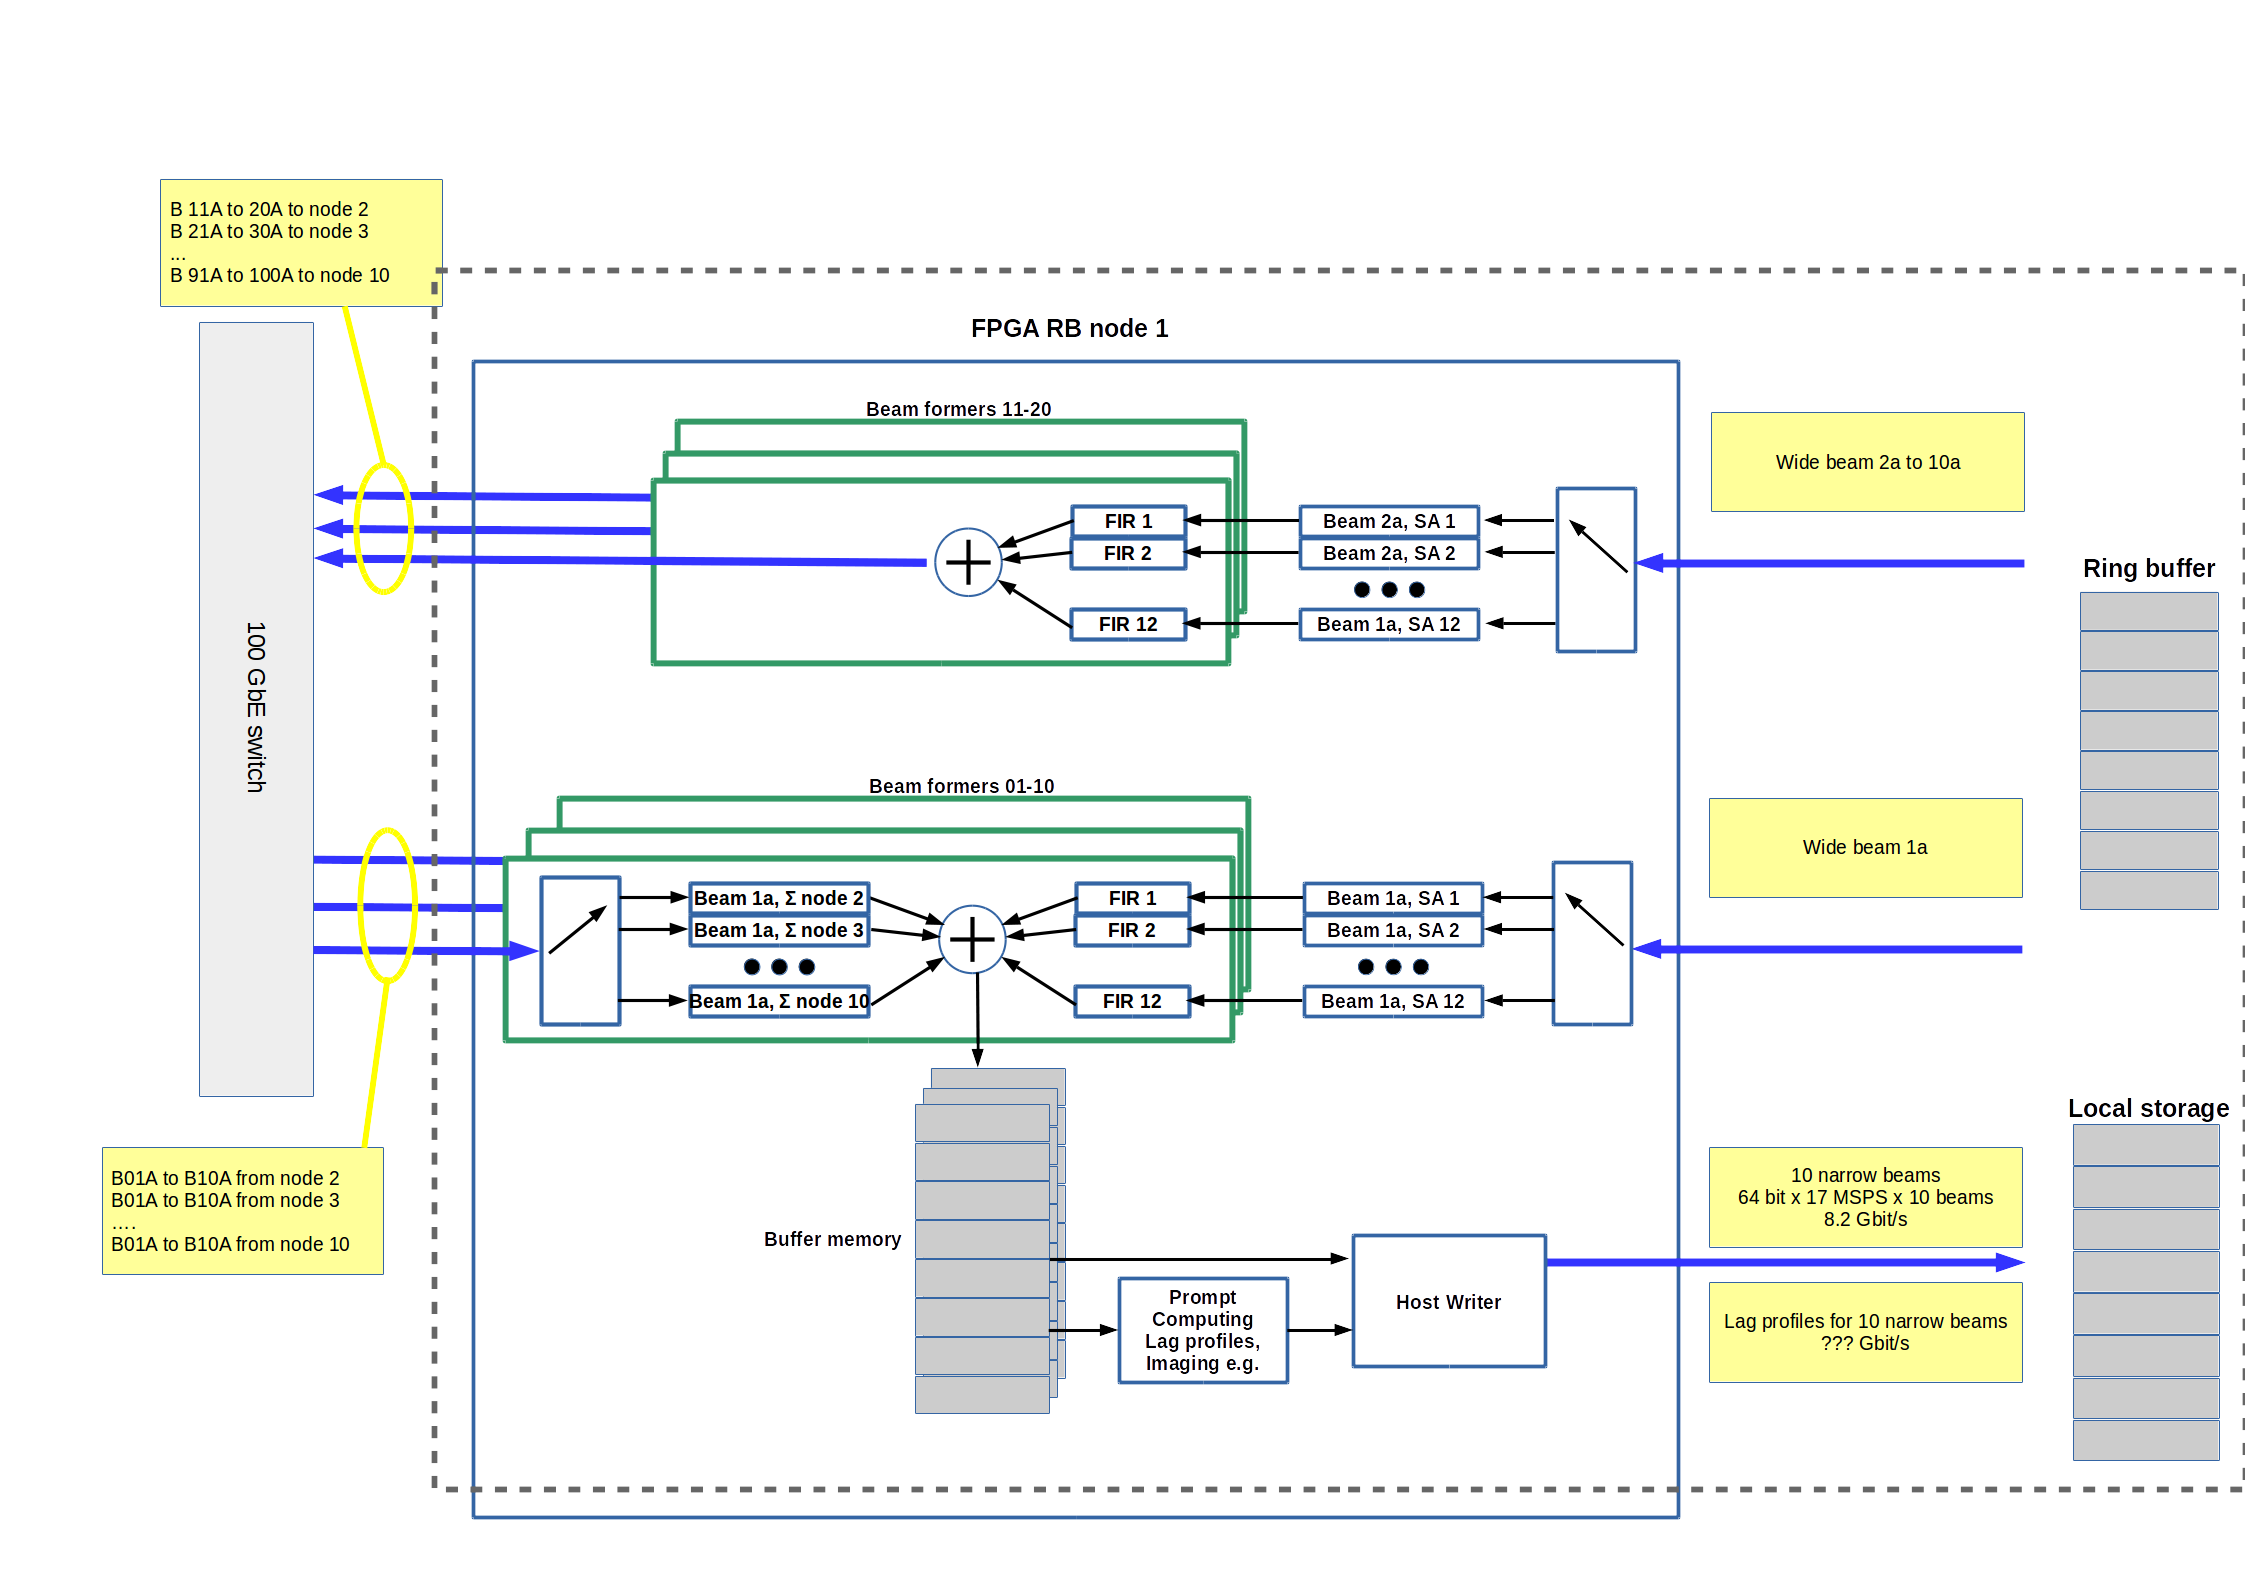
\includegraphics[scale=0.3]{E3DDS_D2_sbf_fpga.png}

FPGA or GPU cards can be used as an optional accelerator for prompt computing or correlators for imaging experiments. 
Accelerator cards should be connected together using fast network or direct card to card (e.g. NVLink) connections.
\fi

% \subsection{Beamforming benchmarks}
% The benchmarking of the beamforming software and testing on the AMD server are still ongoing.
\section{File Writer}
\label{sec:filewriter}

As described, it must be possible to write both raw \RB data and the up to \NNB narrow beams to disk, with a bandwidth of at least \NBW in the first stage of the \ED implementation. 
 The raw complex IQ domain voltage data shall be kept in online storage for reanalysis for a limited time, after which a certain fraction of interesting raw data shall be selected for permanent archival.  
 
 It is thus necessary to implement dedicated file writer processes. These file writers will be triggered by the radar controller based on events in the event list, waking up when data from a certain experiment/beam combination should be written. 

The fast saving mode from FSRUs is a similar operation as the file writing after SBF. 
The same mechanisms for file catalogs and transfers to the data center can be used. 
Also in case of 20 RB nodes write speeds from both sources are very similar and same type of hardware is required. 
It could make sense to use the same devices for both functions so that storage space can be used flexible depending of operation modes. 

Issues to determine include whether separate cluster nodes would be required to run (some of the site beam) file writer processes and the format and granularity of the files. 
The file format is open, but it is foreseen to use the \HDF~\cite{hdf} library to write files for archival, so it would be natural to use \HDF even in the first stage of raw data.


\subsection{File writer capacity requirements}
The main part of the file writing capacity will be used for raw data storage. The highest real-time data rate after Second level Beamformer is when parameters are:
\begin{itemize}
\item 100 narrow-angle beams;
\item 2 polarization each;
\item 2 x 32 bit float samples; % Question from Anders about when these are transformed to floating point? JSW.
\item 6.5 MSPS sampling rate ( 5 MHz analog band width).
\end{itemize}

This gives a total data rate of 10 GByte/s. Fastest SSD disks have continuous write rates of around 2 GBytes/s. Further testing is needed to check if file writing HW and SW can be added to the Ring Buffer Nodes. In the case of 20 Ring Buffer Nodes raw data stream into one SSD is at maximum 0.5 Gbits/s and having 2TB capacity a buffer of 40TB can be constructed. This gives us about 1 hour operational buffer storage in each site.  

\subsection{File format details}

\HDF is a container format whose content is flexible. An open \HDF file presents a directory-like structure through the high-level API. The library is written in \CP with interfaces to Python and several other languages, including proprietary ones such as Matlab, which covers all foreseen \ED use cases. 

Whereas the \HDF library presents a high level view of the data, the actual data written to disk are sorted in a B-tree structure for fastest random access. Several storage backends are selectable. Features including data chunk sizes, bit shuffling and compression of data can all be tweaked through the API.

An example of an existing \HDF implementation for storing radar data is \DRF, developed for the Millstone Hill radar of the MIT Haystack observatory near Boston. This is a straightforward \HDF format intended for continuously streaming samples.  The basic idea is to index samples by UNIX time. The format is used at several radars and the code is available on Github~\cite{drf}.

The structure of a \DRF archive is outlined below.  Note that there has to be one top level directory per sample rate in order for the simple indexing by time to work. The end user does not have to see this structure since the API takes care of indexing by channel and sample.

\vspace{0.4cm}
\begin{minipage}{\textwidth}

\begin{itemize}
    \item Sample rate 1 directory
    \begin{itemize}
        \item Channel 1 subdirectory
        \begin{itemize}
            \item time1.hdf5
            \item time2.hdf5
            \item \ldots
        \end{itemize}
        \item Channel 2 subdirectory
        \item \ldots
        \item Metadata directory
    \end{itemize}
    \item Sample rate 2 directory
    \item \ldots
\end{itemize}
\end{minipage}
\vspace{0.4cm}

\DRF seems to be a possible option for an \ED raw data format. Beams and experiments could be translated to \DRF channels. However, the linear indexing by sample is optimal for continuously streaming data. In \ED it would be more natural to base the storage format on a concept of data blocks.  The hierarchy of \ED files is more naturally

\begin{enumerate}
    \item Experiment (ID, owner, PI)
    \item Beam ID
    \item Data block (\emph{e.g.} samples of one coded pulse)
\end{enumerate}

This hierarchy is easy to translate into an \HDF data structure (as the name implies). 

\begin{enumerate}
    \item Each file corresponds to one experiment ID, known from event list / radar controller state
    \item Each file contains datasets for one or more beam IDs
\end{enumerate}
  The \ED data model~\cite{data-model} has been drafted with these data format and access requirement issues in mind.
 
 \subsection{File writer benchmarks}
% \todo[inline]{Do we have to write something? HH: I don't think we need now}

A plan for benchmarking will be decided, written and performed separately. 
Packets of simulated \fsru data will be generated and written to files, if possible on machines representing all viable options for the site cluster node architecture. 

% CFE: I wrote this but we do not have to specify these here. 
% Issues to decide upon by benchmarking include:
% \begin{itemize}
% \item DigitalRF stream \emph{vs.} data block format;
% \item Multiple beams per \HDF file \emph{vs.} one \HDF file per beam and experiment;
% \item Performance impact of \HDF file chunk sizes, bit ordering, data compression;
% \item Compression in \HDF library \emph{vs.} in backend file system (\emph{e.g.} ZFS);
% \item Metadata in \HDF files \emph{vs.} metadata catalogue;
% \item Using the MPI \HDF library with several processes writing to each \HDF file, \emph{vs.} a one process per file approach;
% \item File system performance, memory mapping of \HDF files;
% \item Lag profiler working on \HDF files \emph{vs.} on data socket.
% \end{itemize}

\section{Prompt computing}

%% \todo[inline]{Ingemar, What data products are needed (lag profiles, echo detection, something else), how much delay is acceptable?, computing resource estimates, network requirements}

The ``prompt" computing cluster produces data products in real-time for the radar operators and users.
The baseline requirement for the \pc is to produce the data products in real-time for the \NBW operations.
The acceptable latency for production of these data products is sub-seconds, that will allow real-time control of the radar and receiver directions. 

EISCAT provides a set of Common Programme (CP) experiments~\cite{eiscat-cp1}.
The data products for these CP experiments include:
\begin{enumerate}
    \item Lag Profiles / Spectra (Time domain / frequency domain);
    \item Plasma lines / Moments of Spectra;
    \item Plasma Parameters (Density, Temperature and E-Field strength) (fitting);
    \item NEIALs and Ion Lines - from plasma parameters - Requires ring buffer data;
    \item Orbit information for objects deemed allowable to observe... ``whitelisted'';
    \item Meteor data (Range bounded so easy to differentiate from satellites);
    \item Interferometry - Requires ring buffer data.
\end{enumerate}

The previous estimate of the computing resources required for the prompt computing is 55~TFLOPS.
Two very important questions to be answered are 
if the prompt computing can be
performed in a virtual environment and if it can be transferred away from RX~\footnote{Remote (RX) sites have receive capacity only whereas the transmitting (TX) has both transmit and receive capacities.} sites (and TX) to a centralized location.
% receiving data from all RX sites.

\subsection{Lag profiles}

The ``lag profiler'' is a software that takes the 32+32~bit IQ data stream from the SBF and produces data in the power domain.
For the current EISCAT systems, the output lag profile data format is Matlab v4 double complex~\footnote{See Section 4 of \url{https://www.mathworks.com/help/pdf_doc/matlab/matfile_format.pdf}}.
Therefore we make the assumption that the lag profiling for \ED will need to handle (output) the same floating-point precision.

\subsubsection{CPU}

So far, the available lag profile code has only been benchmarked on a high-specification gaming PC.
This machine has a 4.3~GHz~CPU with 6~cores (12 hyper-threads) and is approximated in performance to one-half of a more modern ``Skylake''~\cite{skylake} CPU.
It is observed that the gaming CPU requires 21~s to process 10~s worth of data.

Therefore, a calculation for the amount of computing per \NBW beam is as follows: \\
21~(s$\cdot$Gaming CPU)/ 10~(s$\cdot$beam) $\times$ 0.5 (Skylake CPU/Gaming CPU) $\approx$  1 Skylake CPU/beam

At the Skibotn TX site there are 2 wide-angle beams in the \NBW mode, implying 20 narrow angle beams.
Therefore $\approx 20$~Skylake CPUs are required to process the \NBW lag profiles in real-time.

% \todo[inline]{Could someone explain this sentence below? I don't understand... is this per beam?
% HH:As the Rx beams in remote sites are measuring only part of the Tx pulse line we don't need to sample all the time, thus 25\%. SBF beam is divided into frequency bands and analyzing is done separately for those.  But this means nominal FSRU beam must be at least 20~MHz (and SBF)? 
% Do we have any other name for frequency limited signal than 'beam'? Beamlet maybe?
% In remote:
%    1 beamlet $\approx$ 1/4 Skylake CPU?
%    1 beam $\approx$ 1 CPU?
%    100 beam $\approx$ 100 CPU?}



At the remote RX sites the average receiver duty cycle is 25~\%, vs. 75~\% for the TX site, and 100 narrow-angle beams are produced. The receiver duty cycle based on how long the transmitted pulse is present in a wide angle beam for a remote site, beam width coverage plus transmitted pulse length, and how long a receiving session is for the transmitting site. Therefore:

50 beams $\times$ $\approx 1$ Skylake CPU/beam $\times$ .25/.75 (duty cycle) $\approx$ 17 Skylake CPUs

A minimum requirement for the first years is to run the present Common Program operations at maximum transmit duty cycle. 
These are six different modes~\cite{eiscat-cp1} to fulfill various scientific questions, although one expect that the current CP2 mode will be fulfilled be the \ED CP1 mode. 
The table below shows some realistic, but modest, realisations of these basic modes, and estimates the number of beams with given band widths. 
Here, only Skibotn is supposed to do plasma line measurements, but a few remote beams could also be considered for this. The number of Skylake CPUs are for Skibotn plus two remote sites.

\begin{center}
\begin{tabular}{lcllll}
{Mode}&{TX}&{TX BW}&{RX Skibotn}&{RX Remote} & {Skylake CPUs} \\
 & {Dirs} & & &  & {(Skibotn/Remote)} \\
                CP1 & 1 & 1.3 MHz & 4 + 17 MHz & 40*4 + 10*17 MHz & 5/17\\
                CP3 & 6 & 0.1-0.3 MHz & 0.2-0.6 + 17 MHz & 50*(0.2-0.6) MHz & 2/2\\
                CP4 & 1 & 0.1 MHz & 0.2 + 17 MHz & 10*1 MHz & 2/2\\
                CP6 & 1 & 1.3 MHz & 4 + 17 MHz & 50*4 MHz & 3/17 \\
                CP7 & 1 & 0.01 MHz & 0.1 + 17 MHz & 50*0.1 MHz & 2/2 \\
\end{tabular}
\end{center}               

For CP3, the BWs and number of beams varies depending on the TX beam direction. 
The most demanding mode for the computing is the CP1 mode. Here 5 CPUs at Skibotn and 17 CPUs at each remote site would cover the lag profiling needs. 
As lag profiling is mainly done via FFT, the CPU calculation assumes a NlogN dependence, where N is linear to the band width.
This estimate must be benchmarked and checked for accuracy.
% \todo[inline]{Should we say something about CP5 here? Fore example, CP5 resource needs are assumed to  be small compared to other experiments.}
%% CP2. IH: Don't really need for E3D.


\subsubsection{GPU}

A further lag profile benchmark was run on the same gaming machine (4.3~GHz CPU with 6~cores), equipped with a consumer-grade GPU-card.
It was observed that the 10~s of data was processed in 8~s.
GPUs can process the \NBW lag profiles in real-time.

The current estimate is that one consumer-grade GPU per beam at the TX site and one per three beams at the RX site would be required.

\section{Data storage and transfer}
\label{sec:storage}
%Just a reminder, to be removed later
%\emph{Author(s): Mattias}

%(Tests are to be undertaken for this deliverable). 

Data storage and transfer still hold many open issues. 
Different wide-area networking options connecting sites is discussed in detail in revised version of document~\cite{e3dds-del1}. 
At the moment the following scenarios are considered:
\begin{itemize}
    \item Only FSRUs are on RX sites; 
    \item all capacity required by prompt computing is at RX sites.
\end{itemize}
The first option would mean that the file writing would be centralised to one place, which could be the core Skibotn TX/RX site or a HPC centre.
%operation and data centre(s). 
This would be  advantageous with respect to operation and maintenance and it would most likely decrease the number of necessary visits to RX sites as to be discussed in the update to~\cite{e3dds-del1}.
On the other hand, it is also possible that archive-format files will be generated and curated on-site. 

The network solution does not change the service architecture much. 
Ring buffer will be needed, \SBF{} functionality will be needed, files will have to be written into storage devices, and datasets will have to be formed from individual files. The only difference is that the distance between certain system components may be couple of hundred kilometers.

Figure~\ref{fig:dataflow-overall} shows the flow of data from production at the sites to user analysis and publication of results. 
Required services are data archives, a user authentication and authorisation infrastructure (AAI), and facilities for publishing data with unique persistent identifiers. These will be described below. 
\begin{figure}
    \centering
    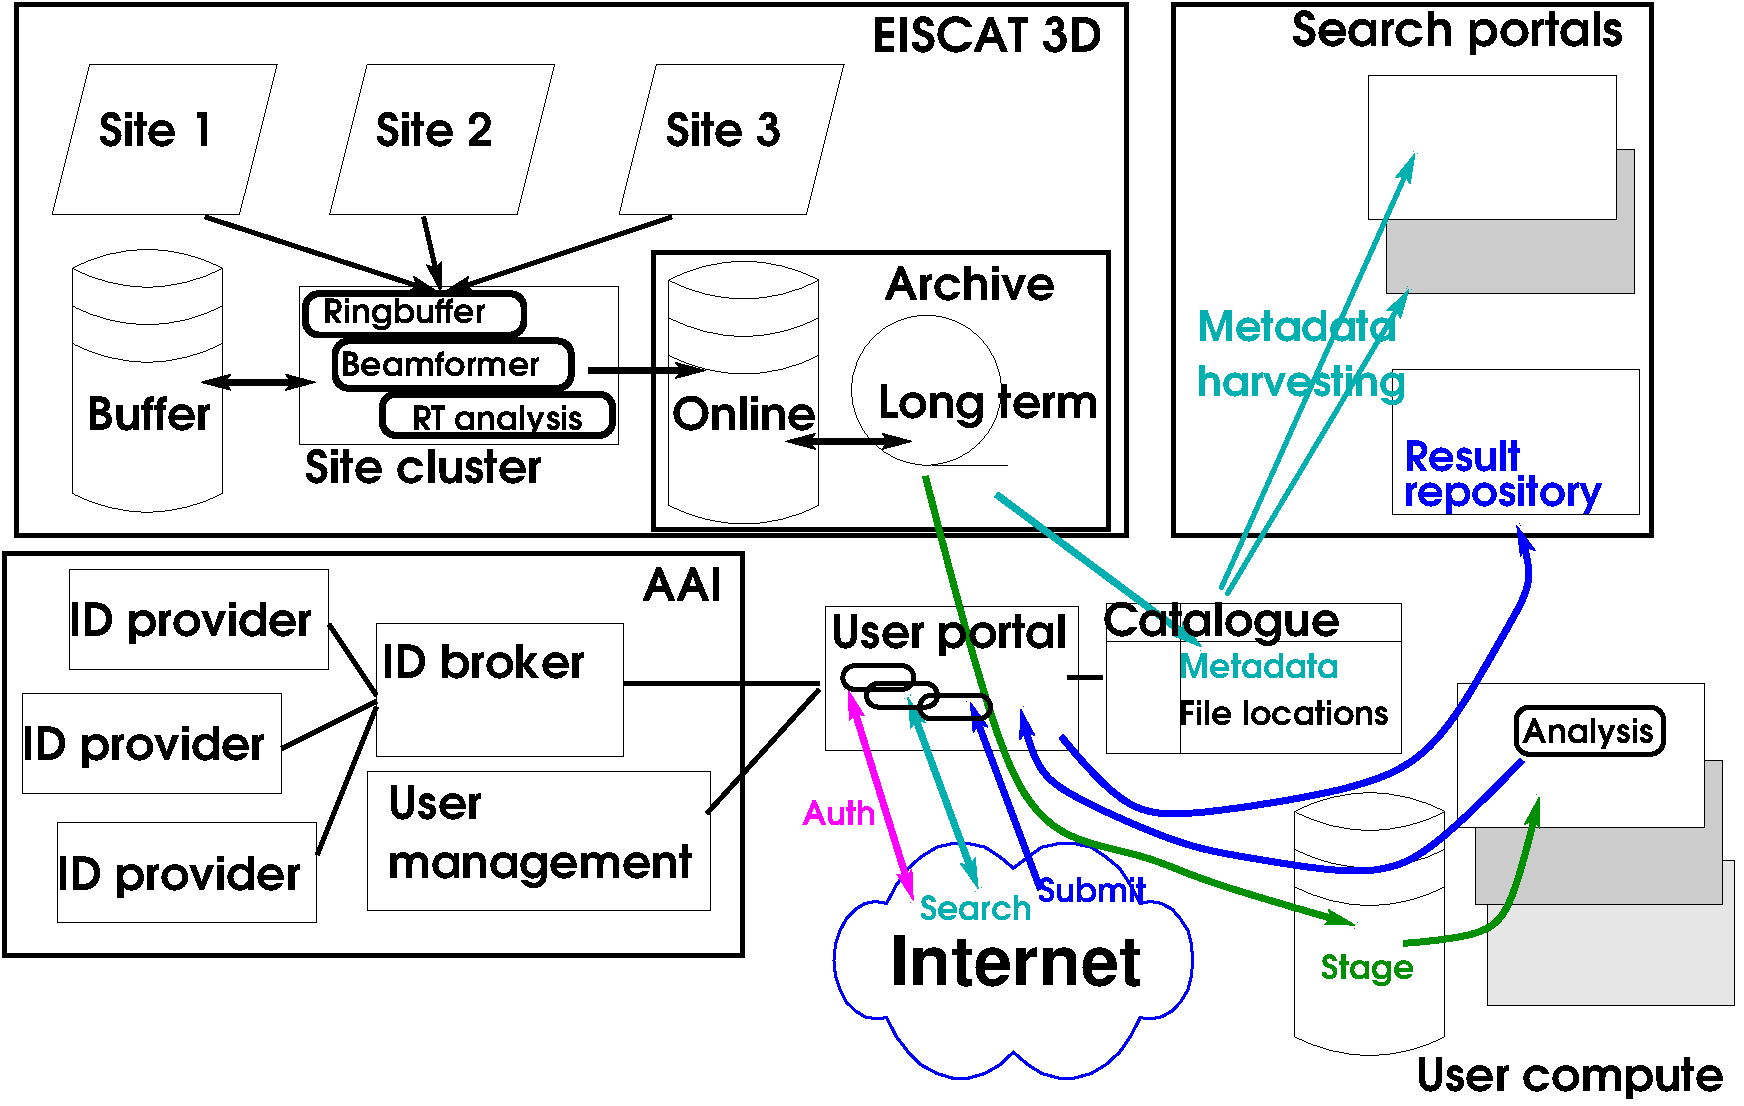
\includegraphics[width=\linewidth]{E3DDS-D2-dataflow.pdf}
    \caption{Data flows in \ED, including data production, authentication and authorisation infrastructure (AAI), user analysis including a data discovery portal and job submission, and publication of results.
    \label{fig:dataflow-overall}}
\end{figure}


\subsection{Site storage}
Files written by filewriter processes will be converted to an archive format by adding metadata, both to relevant metadata records in the actual files and to a metadata catalogue. 
For the on-site (or datacenter) file management, several options are being considered, such as plain file systems, parallel file systems e.g. Lustre~\cite{lustre} or IBM Spectrum Scale~\cite{ibm-gpfs} (earlier known as GPFS), and file and data management systems including dCache~\cite{dcache} and Rucio~\cite{rucio}.

%For the case of files being written into local filesystems as short-term buffers for immediate transfer to other sites, using the ringbuffer nodes for this could be a way to save money over dedicated nodes, given that the CPU and IO load is not too great for the combined functions.

The role of each service component in data chain plays an important role on selection of site storage technologies. The main factors are cost efficiency, fault tolerance and how much data we can afford to lose. 
If there is no unique data stored in site, simple, perhaps somewhat less fault tolerant, service components could be used. 
In such a case, new data would have to be transferred immediately from sites to data centers.
Local filesystems in the RBBF nodes could perhaps be used as a cost effective short-term buffers for data that has not yet been sent forward. 
This approach would require the that there are be enough CPU and I/O capacity in the RBBF nodes for combined functions.

In case the data processing is done in a centralized location, more or less identical data availability risk and risk mitigation possibilities will have to be considered. 

\subsection{Data transfer from sites}

Selection of data transfer tools and protocols to move data between and from sites will be somewhat affected the chosen networking technology. 
If data products are to be computed on all sites, data files will have to be transferred both between the receiver and transmitter sites (for multistatic operation) and eventually to operations and data centres. With the currently proposed dedicated optical link configuration, only Level 1a data will be transferred as UDP packets between sites during operation, but data products will still have to be copied out of the main site as collections of files.
For these purposes there are several suitable file transfer protocols: NFS, GridFTP, HTTPS/webdav,~\emph{etc.}  It should be noted that the volume of data produced will make this a challenging problem.  Therefore, file transfer between distant locations has been tested (see below).

%In the second scenario, \emph{i.e.} only the \fsru{}s are on the remote sites, raw data %(level 1a) will be streamed to the central site using the UDP protocol.
% \todo[inline]{Assuming that we will have computing capasity on sites, do we really have to transfer data between sites ? }
%According to the current plan, there will be a fibre-optic ring connecting the TX and %RX-sites. 

The total throughput of the optical fiber connections will likely be 100 or 200 Gb/s bidirectionally. 
Whatever data transfer practices are needed, the total amount of traffic between \ED sites cannot exceed this given maximum capacity. It should be noted, however, that it would be possible to increase the maximum bandwidth at a relatively small cost compared to the base investment of \ED.

\subsection{File transfer tool benchmark}
% \todo[inline]{should we clarify that "Sustained rate of up to 60~Gbit/s" can not be achieved simultaneously from all sites ? }
There has to be a reliable and fast mechanism to move (and replicate) \ED data products to archives and user analysis computing. 
Therefore, tools to manage data transfers are being evaluated and different methods to move data between sites tested.

Possible candidates for data management tools are \emph{e.g.} Rucio and DIRAC. Possible file transfer protocols are \emph{e.g.} GridFTP and http/https.
The file transfer benchmark should evaluate the performance, usability, and reliability of these tools used to manage data transfers using given transfer protocols.

%he final target should be to reach real-time full bandwidth data transfer from each %site,~\emph{i.e.} a sustained rate of up to 60~Gb/s (plus file, metadata, network and %other overhead) from each remote site to a central location. 
%However, this requirement will most likely be relaxed by the on-site file buffers.
%\subsubsection{File transfer tests}
%\label{ssec:file-tr-tests}

Such file transfer tests have been performed between sites with high-speed connections to the Nordic NRENs.  The E3DDS project was granted storage on Swestore (SNIC allocation 2018/12-18).  This is a distributed dCache system with access through WebDAV, and GridFTP (and possibly more exotic protocols like xrootd should it be required). 
On top of Swestore we deployed an instance of Rucio and replicated sets of existing EISCAT data or big random files. Results from these tests are available at the NeIC web page {\url{ https://wiki.neic.no/int/E3DDS_Data_Transfer_Tests}}.

%, a data management system that originated from the LHC ATLAS experiment. 
% \todo[inline]{Link to Vincent's presentation here}

% Notes: dCache is mainly Java, Rucio and DIRAC mostly Python. Are there more efficient solutions? Converting DIRAC to Go for better parallel performance was discussed some time ago, as an idea for future developments. The dCache.org team seems capable of writing high performance Java for the most part though, CPU pefromance is seldom an issue for NT1 operations (which is currently in the 60Gbit/s range).

\subsection{Metadata management}

Metadata of \ED experiments will be registered in one or more databases as necessary, including schedule, file catalogue, and relevant information for the master event list. Figure~\ref{fig:dataflow-overall} shows this as one catalogue, which in practice can be any number of SQL or NoSQL databases. In the EOSC-Hub CC for \ED, the DIRAC interware, originating from the LHCb detector, is being adapted for \ED data.  The DIRAC file catalogue will be required to store sufficient metadata for users to search. 
 Additionally, individual data files will contain basic information including start time, stop time and type of data. 

Metadata and data archival should adhere to the FAIR principles (Findable, Accessible, Interoperable, Reusable). 
The \ED project is one of the Atmospheric Research infrastructures participating in the ENVRI-FAIR H2020 project~\cite{envri-fair}. 
The ENVRI collaboration provides guidelines on common solutions to issues of data sharing and metadata. 
It is planned that \ED will expose DataCite and possibly INSPIRE metadata for harvesting. 
The metadata management thus has to be based on flexible metadata schema management tools. 
It should expose an OAI-PMH~\cite{oai-pmh} API for metadata harvesting purposes.

Separating the metadata master repository from other tools such as DIRAC and external search engines will enable the roles of these services to be clearly separated to front-end and back-end services.  
This, in principle, will provide better IT security and it will also allow EISCAT to change service components should it be necessary. 

%\ED-specific metadata will include at least
%\begin{itemize}
%    \item Experiment time
%    \item Experiment owner, for access control %according to EISCAT rules
%     \item Experiment configuration %\cite{data-model}.
%     %\url{https://wiki.neic.no/wiki/EISCAT_3D_D%ata_Solutions\#EISCAT_3D_Data_Model}}
%\end{itemize}

The generic \ED metadata schema should take into account the requirement to translate to the DataCite metadata schema~\footnote{Schema version 3.1 or newer would be recommended, see \url{https://schema.datacite.org/}}. 
This schema ensures interoperability with EUDAT and OpenAIRE services.
With this in mind we have drafted a specification for DataCite metadata to expose, see \url{https://cryptpad.fr/pad/#/2/pad/edit/5vCPqDOQm0vpZxS3dSYEZwpJ/}
%% Can we get a eiscat.se snapshot of this document?

In addition to the above discussed experiment metadata and generic research data metadata, additional information about the history of dataset creation should be recorded, i.e. provenance and versioning.
This is important, because only with the help of such additional information it is later possible to find out possible impact of 
\emph{e.g.} error prone numerical libraries
or faulty hardware. 
It is not easy to collect all the information, but the list below contain some elements that could be considered to be stored to metadata catalog and linked to datasets:
\begin{itemize}
    \item Hardware (generic level, hardware set level, individual item level),
    \item Operating system (major version, minor version, patch release), 
    \item Configuration (what is the configuration item?)
    \item Middleware (\emph{e.g.} docker version)
    \item Application (major version, minor version, release)
\end{itemize}
In practice, the list also says that \ED{} software development and data analysis  practices will have to be defined and later also followed.

There are couple of possible choices for metadata management solutions, for instance CKAN~\cite{ckan} and Invenio~\cite{invenio}. 
These will likely be used anyway in the \ED data workflow since B2SHARE, which can be used as a repository for analysed results, is an implementation of Invenio, and B2FIND, where the DataCite metadata will go, is based on CKAN. 
These may be too inflexible tools for pure internal metadata management purposes though. 
Therefore the use of common databases with necessary add-on tools (web access, Elastic Search, \emph{etc.}) may have to be considered. 
More detailed requirements,~\emph{e.g.} scalability in terms of number of datasets, performance requirements,~\emph{etc.} will have to be defined independently of the metadata management tool.

\subsection{Persistent identifiers}
Published data should include globally resolvable persistent identifiers. 
DataCite mandates the use of DOIs~\cite{doi} and will be used for the top level data collections of \ED data, corresponding to scheduled experiments and/or published data.
At lower levels of data, other PIDs such as ePIC handles~\cite{epic} are considered for unique identification of datasets.

Before data publishing, for data management purposes, internal non-resolvable identifiers should also be considered.
An obvious choice for such an identifier would be universally unique identifier (UUID). 
Because UUIDs can be created in distributed environments, a logical choice for UUID generation would be the file writer component discussed earlier in Section~\ref{sec:filewriter}.

%% \todo[inline]{Mention the FREYA project? https://project-freya.eu/en }

%When data is published, published datasets %should contain globally resolvable persistent %identifiers. Possible candidates are \emph{e.g.}% Handle software based %ePIC~\cite{epic} and DOI~\cite{doi}. 
%The latter one has recently gained lot of %popularity and it is often required to be used %with scientific publications. 
%DOI and ePIC are also recommended by the %ENVRI-FAIR project. 

Handle system-based persistent identifiers may contain additional metadata, that can be used to find the right dataset.  
The policy in DOI identifiers is that the identifier should point to a landing page giving more information about the data collection. 
The source of this information  should be the master metadata repository used by \ED.

Handle-based identifiers consists of a prefix, specific to each organisation, and a suffix, which is an arbitrary string following a specified format. 
Handle based system provide a possibility to use fragments (or template handles, as described in the Handle manual), to allow more fine grained access to dataset objects. 
However, it should be noted, that no standard how fragments are used or handled on service side exists. The logic is service specific --- it has to be done on service itself by the service itself. 
In practice, this means that if data are later moved to another service, this same operational logic should also be implemented there. 
%In this way, handle-based identifiers can contain metadata information about the objects they refer. 
EISCAT should ensure that data can be easily moved between services by EISCAT itself. 
In practice, this means that EISCAT should have its own prefixes for DOI and other used PIDs. 
All EISCAT data should thus be under one (or more) prefixes that are solely used to store EISCAT data. 
This is because, in persistent identifier systems, access rights are not managed on individual identifier level but the higher prefix level. 
A DOI prefix will be obtained by membership in DataCite.

\subsection{Data Centres}

Data centres receive data from remote sites. They also provide online copy of most recent data objects and archive copy of all data objects. 
dCache and Rucio are potential candidates for data management tools managing data transfers between RX sites and data centres. 

Online data service should provide fast access to most recent data. Archive copy service should ensure that data is safely stored in an environment able to guarantee long term data preservation.
To ensure maximum data availability, 
archive copy should be done immediately when data is ingested to datacenter. 

Use case and storage technologies used set some guidelines for selecting the size of a data object. Online datasets should be large enough, so that number of files would not be too high. On the other hand, dataset size should not be too large, because it would complicate data downloads. On storage technology point of view, object storage services would prefer object sizes smaller than 5~GB, because datasets smaller than  that can be stored in one object storage object.
Tape based storage systems can in principle handle larger objects, but in practise accessing and managing files of size 1~TB or so may be slow. 

Open Archival Reference Model (OAIS)~\cite{oais}, that has been published as an ISO standard 14721, defines the reference model for an open archival information system. This model is most likely a bit too complicated to be used
for \ED{}, but at least following principles should be followed:
\begin{itemize}
    \item Used file formats should be well documented and open;
    \item Validators should be used to check that archived packages are properly built;
    \item Metadata is well defined, versioned, and stored with data;
    \item Integrity of archived data is monitored.
\end{itemize}
In the evaluation done by \emph{The Open Science and Research Initiative}, different file formats used to store scientific data were studied. 
The study~\footnote{\url{https://avointiede.fi/sites/avointiede.fi/files/research\%20data\%20file\%20formats\%20Final\%20report.pdf}} concentrated on evaluating how good candidates these formats would be for long term preservation. 
The report states that HDF5 was found to be open and documented, maintained by a non-commercial organisation (HDF Group). 
It was also "mostly" both down and upwards compatible within the different versions of HDF5. 
In addition, HDF5 is supported in many different software packages, although these packages do not necessarily support all the HDF5 features. 
The format was internationally approved as a recommended or transferable format in some reputable organisations (CINES, DANS, US Library of Congress).


\subsection{End user portal}
% A very short description of DIRAC GUIs

End users will interact with the metadata catalogue, file archives, and analysis computing through a user portal. As shown in Figure~\ref{fig:dataflow-overall} it has to be accessible from the public Internet but only allow access to authorised users. 
The \emph{EOSC-Hub EISCAT CC} -project is adapting the web GUI of DIRAC~\cite{dirac} for this purpose. 
The prototype is accessible~\footnote{\url{https://dirac.egi.eu:9443}} with authentication by EGI Checkin or through X.509 based VOMS user registration. 
This portal presents a desktop-like user interface with several applications. 
The most important available applications are proxy upload, file catalogue, job submission, and job management. 
Examples of the DIRAC portal and how to use it are collected at the EISCAT web page~\cite{eiscat-dirac}.

More advanced use of DIRAC is possible through the DIRAC CLI, which is installable as well as available as a Docker image.

\subsection{Data publishing}

%DIRAC seems to be an obvious choice for end user analysis purposes, would it be a good  candidate for 
% data publishing too. 
Data used for scientific work will have to be citable in publications in the same way as scientific articles.
The data services of \ED should create  persistent identifiers and landing pages for persistent identifiers, provide a public metadata catalog, provide a metadata harvesting API \emph{etc.}  Data objects have to have persistent identifiers pointing to landing pages. 

%For data publishing purposes Invenio, or perhaps also CKAN, could be reasonable alternatives. In EUDAT, Invenio is used in the %B2Share service as a tool providing data publishing service. \todo[inline]{Recommended approach is to assing PIDs to data %queries, are these systems compliant with that approach? Also, these queries will have to resolve to the (meta)data (landing %pages?) for an indefinite future\ldots \\
%COMMENT: PIDs for queries have been discussed in RDA dynamic data recommendation. If the data is static, are there reasons to %have  citable queries, because datasets can be cited directly. Or is there a need to be able to create citable datasets %consisting of already existing datasets?}

For identifying published data collections we will very likely use DataCite. DataCite mandates the use of DOIs as identifiers and specifies a limited number of other required metadata fields according to a not very complicated vocabulary.
Therefore a natural approach is that once a user has accepted any number of data products for publication, a citable data collection should be created. 
\begin{enumerate}
    \item Share result entry on B2SHARE (an instance of Invenio). Collection of data to cite is defined by a database query.
    \item B2SHARE entry gets DOI and is harvested to other search systems as well.
    \item DOI resolves to B2SHARE as landing page.
    \item Data query should also include version of files. Any reanalysis should create a new version, not overwrite files.
\end{enumerate}
This is the process indicated by the blue arrows in Figure~\ref{fig:dataflow-overall}.
The same procedure of creating a top level data collection will also apply to standard \ED experiments which are likely to be cited as such. There will thus be both automatically created and user-defined data collections identified by a DOI.

It should be noted, that although the FAIR principles and an open data policy are strongly favoured, all data do not have to be public. However, all published data should have public metadata. Access to data can be available only upon request. In addition, according to EISCAT statutes, data embargo times apply. Data embargo may have set practical requirement to 
persistent identifier systems, because identifiers are usually needed also for embargoed datasets.

\section{Multi-site cluster control}
% Describe tools used to ensure that computing clusters and storage systems have right configuratins, are properly mainteined, and monitored
% This can be merged with next chapter and do Cluster Management?
The expected number of servers on the 3-5 remote sites is inversely proportional to the capacity of the wide area network (WAN).
With a low-capacity (100~Gb/s or lower) WAN, it will be necessary to locate the 10~RBBF nodes on remote sites. 
The prompt computing could be sited at a central site.
A high capacity (multi~Tb/s) WAN, would allow all remote site computing to be located centrally.
A full optical multe-Tb/s WAN would allow a remote site computing configuration consisting only of FSRUs and timing distribution server(s). 
% This will affect the selection of the cluster management tools.

\subsection{On site management cluster}
\label{sec:onsitemanagementcluster}
%Possible tools for management cluster
If an on-site management cluster is required, it must be able to run all essential management software at the site. Possible candidates are \emph{e.g.} KVM, Xen, and VMware based solutions. 
The mandatory requirement for virtualization platform is that system administrators must be easily able to migrate services from one host to another. 
A subsequent requirement is that service migration can be done on fly without a service break. 
At the moment, there are no plans to install any shared storage system on site. 
Therefore, the management cluster nodes should be able to replicate data between nodes.

\subsection{Cluster management tools}
\label{ssec:clust-manag}
%Possible tools for management cluster
In addition to these servers, there may be additional physical or virtual hosts in national service providers premises, in datacenters storing \ED data, and in the \ED operations center.
Depending on the usage pattern, additional computing capacity could also be made available using cloud services. 
To ensure that the whole research infrastructure used by \ED will be able to provide required services in a reliable and documented way, the whole infrastructure will have to be managed in a consistent manner. 

There are number of tools used to maintain computing clusters, for instance, Ansible~\cite{ansible},
xCAT~\cite{xcat}, OpenHPC~\cite{openhpc}. 
Whatever set of tools will be chosen, the environment should be defined in such a way that, it can be maintained, reinstalled, and even relocated with minimal work.

\subsection{Software distribution}
%CernFS

To share configuration files, containers, \emph{etc.} to remote sites, a  service synchronizing files and directories is needed. 
In principle, this could be done by \emph{e.g.} rsync, but a distributed filesystem like CernVM File System~\cite{cernvmfs} could also be used. 
A software repository tool, such as GitLab~\cite{gitlab}
or similar, accessible from all \ED nodes will also be needed.

% TODO something about DIRAC client for distributing software

\subsection{Monitoring and capacity management}
%Monitoring tool(s), log analysis tools, Dashboard about metric

All IT infrastructure in the \ED service production should be monitored, so that incidents could be detected and incident resolution process could be started as quickly as possible. Therefore, a monitoring tool is needed. 
This tool should be able to provide an easy to follow dashboard that clearly shows, by using e.g. different colours, what services are working within normal parameters, what services are working below normal parameters and what services do not respond at all. 
In addition, time series information about service availability, service and service component  capacity, performance, throughput, \emph{etc.} has to be collected into tool enabling system administrators to diagnose the status of the service and to do capacity management tasks.

\ED servers will generate log files, that should be collected by a dedicated tool such as {Logstash}~\cite{logstash}. 
This tool should do continuous analysis using predefined filters about logs and, if necessary, inform the monitoring system that there are events requiring further analysis.

Tools described above are necessary for  in incident management process.
They should be be functional in all reasonably expected incidents including power distribution failures in the remote sites. 

Monitoring and log analysis information form a basis for
operator displays, \emph{i.e.} standard views that operators use to ensure that the overall status of \ED is within normal parameters. 
The exact information needed for operator displays will be defined later.

\subsection{Emergency shutdown}

The computing capacity, especially on the RX sites, will produce heat. 
The exact amount of heat is not precisely known at this time but this heat must be removed from server room to ensure that the systems can operate normally.
In case there is a problem with the cooling, the room temperature increases rapidly. 

The cooling failure risk mitigation should be
taken into account for the site electricity design.
Software controlled ``soft'' power-off would 
give more time for operators to react to an 
incident. 
Graceful power-off would also 
keep file systems, and the data located in filesystems, 
in good condition.

\section{Secondary usage}
%Just a reminder, to be removed later
%\emph{Author(s): Ari}

In case the usage profile of the radar is such that
it will leave a large amount of free CPU cycles in the online data processing chain, the possibility to take these cycles into secondary use may be worth considering.
Unfortunately, these free cycles can not be taken into use without a cost. 
This section discusses some of the issues that should be taken into account, in case unused CPU cycles would be taken into use for generic simulation or analysis tasks.

\subsection{Identity management, access rights, and resource quotas}

Depending on hardware architecture, the RX sites may contain storage devices in the RBBF nodes using disks.
If end users are given access to computing resources, access rights to those data objects should be defined and maintained in such a way that access rights would be respected by all secondary usage processes.
The same is true also for data objects created by end users. The easiest way to manage access rights, would be to use UNIX user and group information. For this purpose, a directory service, like OpenLDAP, would most likely be needed. 

In case the number of users would be more than a few, there might be a need to define resource quotas for CPU and storage resources. 
There should also be a mechanisms collecting information about resource usage and preventing users or projects from exceeding their quotas.

\subsection{Software stack}

Generic computing cluster may contain lot of software that will have to be installed and maintained.  
For maintenance purposes, the use of a software build tool such as EasyBuild~\cite{easybuild}
or Spack~\cite{spack} would be worth considering. 

Instead of installing additional software to all computing nodes,  alternative approach would be to use container tools, \emph{e.g.} singularity. 
It is not clear, however, how well containers would work with parallel computing libraries, should they be needed.

\subsection{Batch queue system and job submission}

Computing cluster contains login nodes, that are connected to Internet and to actual computing cluster. These login nodes are used to compile codes and to launch batch jobs. In the \ED environment, login nodes could locate in virtual nodes within the maintenance clusters. 

Independently of the access method discussed above, a batch queue system would be needed. Commonly used batch queuing systems are \emph{e.g.} Slurm, PBS Pro commodity edition, and the commercial product IBM Spectrum LSF. 

The batch queue system should be connected to the \ED radar controller, because if the CPU cycles are needed for primary purposes, 
the radar controller has to have a possibility to quickly kill or stop all batch queue jobs. In such a case, it would be convenient, if the jobs could be easily restarted, when free CPU cycles would again be available.

A slightly different kind of approach to use free CPU cycles, could be made possible by connecting login nodes directly to DIRAC portal. 
DIRAC works by submitting pilot jobs (python scripts which provision and start analysis processes) and this works with several computing approaches including batch queues (\emph{e.g.} Slurm~\cite{slurm}), cloud compute (such as OpenStack~\cite{openstack}) or plain SSH connections. 
This would be very convenient from the end user point of view. 
On the other hand, it would also provide a rather direct way from a service available to Internet to the very inner core of the operational \ED infrastructure. 
Pros and cons and possible risk mitigation policies of this approach should be considered  carefully.

\newpage
\bibliography{main}{}
\bibliographystyle{unsrt}

\end{document}